% !TEX program = pdflatex
\documentclass[11pt,a4paper]{article}
\usepackage[T1]{fontenc}
\usepackage[utf8]{inputenc}
\usepackage{lmodern}
\usepackage{textcomp}
\usepackage[italian]{babel}
\usepackage{amsmath,amssymb}
\usepackage{graphicx}
\usepackage[a4paper,margin=2.4cm]{geometry}
\usepackage{array}
\usepackage{xcolor}
\usepackage{hyperref}
\usepackage{float}

% --- sostituti minimi di siunitx e booktabs (non inclusi nella distribuzione) ---
\providecommand{\toprule}{\hline}
\providecommand{\midrule}{\hline}
\providecommand{\bottomrule}{\hline}
\providecommand{\micro}{\textmu}
\providecommand{\degreeCelsius}{\textcelsius}
\providecommand{\SI}[2]{#1\,\text{#2}}
\providecommand{\num}[1]{#1}

\hypersetup{colorlinks=true,linkcolor=blue!55!black,citecolor=blue!55!black,
  urlcolor=blue!55!black,pdftitle={Motore Fotonico del Vuoto V6},
  pdfauthor={Francesco Bulla}}

\renewcommand{\figurename}{Figura}
\renewcommand{\tablename}{Tabella}
\renewcommand{\refname}{Riferimenti}
\setlength{\parskip}{0.35em}
\setlength{\parindent}{1.2em}

\title{\bfseries Il rotore otticamente guidato\\[0.3em]
\large Limiti di coppia, dissipazione e stabilit\`a nel Motore Fotonico del Vuoto\\
\large Revisione V6}
\author{Francesco Bulla\\ \small Catania, Italia}
\date{28 ottobre 2026 \quad \small versione 6.1}

\begin{document}
\maketitle

\begin{abstract}
\noindent
La V6 non aggiunge parti alla V5: toglie le ambiguit\`a e mette il modello in
condizione di essere smentito. Il lavoro si regge su tre scelte. La prima \`e un
modello unico, dichiarato come \emph{limite}: $\tau=(\ell+s)P_{\rm ass}/\omega_{\rm
ott}$ e $F=I\sigma_{\rm pr}/c$, due canali distinti e non due modi di dire la stessa
cosa. La seconda \`e un attrito dichiarato come \emph{intervallo}, delimitato dal
teorema di dissipazione minima e dalla teoria dei corpi snelli. La terza \`e che ogni
numero del testo viene da un file di dati generato dal codice accluso.

Questa revisione 6.1 corregge cinque errori della 6.0, tutti materiali. I raggi dei
fili sono quelli della scena V5 (3,2 / 7,5 / 4,5 nm di diametro 6,4 / 15 / 9 nm) e
non 1,25 nm: poich\'e in Rayleigh $\sigma\propto a^2$, le sezioni crescono del 47\,\%
($\sigma_{\rm pr}=1{,}065\times10^{-14}$\,m$^2$ contro $7{,}259\times10^{-15}$) e la
massa passa da $2{,}78$ a $8{,}21\times10^{-18}$\,kg. L'area radiante \`e la
superficie metallica reale ($2{,}69\times10^{-13}$\,m$^2$), non l'inviluppo sferico,
e in vuoto il rotore fonde gi\`a a \SI{1}{\micro W}: \SI{2250}{K} con
$\epsilon=0{,}03$, \SI{1505}{K} con $\epsilon=0{,}15$, contro \SI{1358}{K} di fusione.
La soglia di fusione \`e \SI{0.13}{}--\SI{0.66}{\micro W} di potenza incidente \`e il
tempo adiabatico \SI{0.28}{ms}. Il confronto a pari massa \`e riformulato in modo
condizionale: per l'attrito il risultato \`e robusto (tre decadi di variazione), per
la coppia dipende dalla sezione di forma, che un calcolo DDA deve ancora fornire. Il
confronto con la silice a 1--6\,GHz diventa un controllo di compatibilit\`a sulla
scala meccanica: le coppie $(f,r)$ osservate implicano una tensione efficace fra
$0{,}22$ e $7{,}8$\,GPa, che \`e l'ordine di grandezza della silice su nanoscala, e
nulla pi\`u. L'OAM, infine, non \`e un moltiplicatore: includendo la sovrapposizione di
modo il guadagno netto a $\ell=5$ \`e $1{,}05$, non $6$.

Il risultato che regge a tutte le correzioni \`e che, a \SI{1}{\micro W} in acqua, la
coppia ottica vale $Pe_r=7{,}7\times10^{-4}$ e l'attrito del telaio supera di 209
volte quello del solo nucleo: il rotore non \`e orientato, e la geometria non lo
salva.
\end{abstract}

\vspace{0.3em}
\noindent\rule{\textwidth}{0.4pt}
\section*{Risultati in otto righe}
\addcontentsline{toc}{section}{Risultati in otto righe}
\begin{enumerate}\itemsep2pt
\item \textbf{Raggi dei fili corretti.} 3,2 / 7,5 / 4,5 nm, non 1,25 nm: le sezioni
crescono del 47\,\%, la massa da $5{,}73$ a $8{,}21\times10^{-18}$\,kg, il momento
d'inerzia da $3{,}09\times10^{-32}$ a $4{,}62\times10^{-31}$\,kg\,m$^2$.
\item \textbf{Coppia.} $\tau=3{,}31\times10^{-24}$\,N\,m (+27\,\% sulla V5): usa
$P_{\rm ass}=11{,}70$\,nW e non $P_{\rm int}=13{,}56$\,nW.
\item \textbf{Attrito.} $\beta\in[4{,}04;\,6{,}48]\times10^{-22}$\,N\,m\,s contro
$2{,}89\times10^{-23}$ della V5, che sta al 7\,\% del limite inferiore.
\item \textbf{Figura di merito.} $Pe_r=7{,}72\times10^{-4}$: la rotazione ottica \`e
tre ordini sotto il rumore browniano.
\item \textbf{Termica.} In vuoto, a \SI{1}{\micro W}, \SI{2250}{K} o \SI{1505}{K}
secondo l'emissivit\`a: il rotore fonde. Soglia: \SI{0.13}{}--\SI{0.66}{\micro W}.
\item \textbf{Baseline.} A pari massa il reticolo ha l'attrito pi\`u alto di tutte le
geometrie ($\beta$ da 6 a 98 volte) e la coppia pi\`u bassa (0,44 di quella della
sfera compatta).
\item \textbf{Controllo esterno.} Le osservazioni a 1--6\,GHz implicano
$\sigma_y=0{,}22$--$7{,}8$\,GPa: compatibilit\`a di scala meccanica, non validazione
del modello ottico.
\item \textbf{OAM.} Guadagno netto $1{,}05$ a $\ell=5$: la sovrapposizione di modo
annulla il fattore $\ell$.
\end{enumerate}
\noindent\rule{\textwidth}{0.4pt}

\begin{figure}[H]
\centering
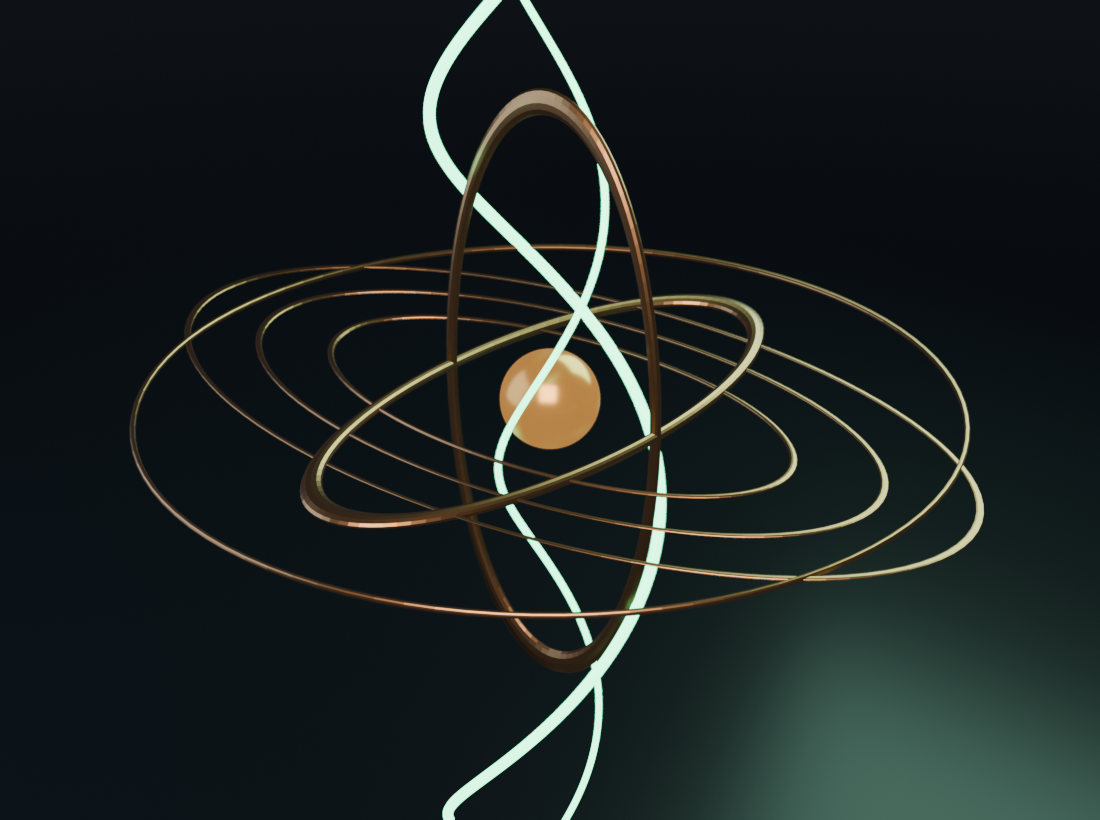
\includegraphics[width=0.86\textwidth]{../blender/rotore_hero.png}
\caption{Il rotore otticamente guidato: telaio di fili, nucleo di rame e fascio con
momento angolare orbitale. La scena Blender \`e costruita con le proporzioni del
modello (1 unit\`a $=$ 100\,nm) e i raggi di filo della V5; il fascio \`e
un'elica, non un cilindro, perch\'e quello che conta non \`e la sua forma ma il
momento angolare che trasporta.}
\label{fig:hero}
\end{figure}

\tableofcontents
\newpage

%=====================================================================
\section{Tesi e criteri di giudizio}
%=====================================================================

La V5 chiudeva con una frase onesta: il modello non rivendica validazione
sperimentale. La V6 parte da l\`i e cambia il criterio di successo. Non chiede se
l'architettura \`e plausibile, ma se le sue grandezze sono compatibili con misure
indipendenti, e a quali condizioni no.

Il titolo \`e cambiato di conseguenza. Non pi\`u \emph{motore}, con la promessa di
spinta che il termine porta con s\'e, ma \emph{rotore otticamente guidato}: un corpo
tenuto e fatto girare da un fascio, del quale si studiano coppia, dissipazione e
stabilit\`a termica. La differenza non \`e nominale. Un motore si giudica dal lavoro
utile; un rotore guidato si giudica da due numeri, entrambi misurabili:
\begin{equation}
\boxed{\;\eta_{\rm int}=\frac{\sigma_{\rm pr}}{A_{\rm fascio}},
\qquad
Pe_r=\frac{\tau}{k_BT}=\frac{\omega_{\rm ss}}{D_r}\;}
\label{eq:merito}
\end{equation}
$\eta_{\rm int}$ dice quanta della luce disponibile tocca la struttura; $Pe_r$ dice
se la coppia ottica sopravvive al rumore orientazionale. Il secondo \`e il numero che
conta: sotto $Pe_r=1$ il rotore non \`e orientato, \`e solo pi\`u caldo.

I quattro criteri con cui va giudicata la revisione sono quelli chiesti in apertura,
e li assumo come impegno: quanto momento angolare la luce trasferisce realmente;
quanto sopravvive alla dissipazione e ai limiti termici; se la geometria
Spin/Contro-spin offre un vantaggio a pari massa; se le previsioni sono compatibili
con risultati indipendenti.

Le risposte della V6 sono, nell'ordine: poco (il limite
$(\ell+s)P_{\rm ass}/\omega_{\rm ott}$, con $P_{\rm ass}$ pari all'86\,\% di
$P_{\rm int}$); quasi nulla (la coppia \`e $10^{-4}\,k_BT$, e in vuoto la fusione
arriva prima dello spin-up); no (il telaio \`e un freno); s\`i, ma solo sulla scala
meccanica. Nessuna delle quattro \`e un fallimento del lavoro: sono il motivo per cui
il lavoro ha senso.

\subsection{Cosa cambia rispetto alla V5}

\begin{table}[H]
\centering\small
\caption{Le grandezze che la V5 dichiarava e il valore che la V6 calcola. Le due
prime righe mostrano che l'errore della V5 non era di modello ma di geometria: con
i raggi di filo sbagliati le sezioni sono sottostimate del 47\,\%.}
\label{tab:confronto}
\begin{tabular}{lrrr}
\toprule
Grandezza & V5 & V6 & causa \\
\midrule
$\sigma_{\rm pr}$ & $7{,}259\times10^{-15}$\,m$^2$ & $1{,}065\times10^{-14}$\,m$^2$ & raggi di filo \\
$F$ & $3{,}083\times10^{-17}$\,N & $4{,}522\times10^{-17}$\,N & raggi di filo \\
$\tau$ & $2{,}610\times10^{-24}$\,N\,m & $3{,}305\times10^{-24}$\,N\,m & $P_{\rm ass}\neq P_{\rm int}$ \\
$\beta$ & $2{,}89\times10^{-23}$\,N\,m\,s & $4{,}04$--$6{,}48\times10^{-22}$ & intervallo fisico \\
$\omega_{\rm ss}$ & $1{,}14\times10^{-1}$\,rad/s & $5{,}1$--$8{,}2\times10^{-3}$\,rad/s & conseguenza di $\beta$ \\
$Pe_r$ & $6{,}10\times10^{-4}$ & $7{,}72\times10^{-4}$ & identit\`a $\tau/k_BT$ \\
\bottomrule
\end{tabular}
\end{table}

%=====================================================================
\section{Chiusura dei residui}
%=====================================================================

Nessuna delle incongruenze segnalate richiede una misura: si chiudono con aritmetica
esatta e con la geometria giusta. La Tabella~\ref{tab:residui} le elenca, la
Figura~\ref{fig:residui} mostra le due pi\`u importanti.

\begin{table}[H]
\centering\small
\caption{Residui e loro chiusura. I valori della colonna V6 sono prodotti da
\texttt{v6\_studi.py}.}
\label{tab:residui}
\begin{tabular}{p{2.9cm}p{3.0cm}p{3.0cm}p{5.5cm}}
\hline
Grandezza & V5 & V6 & nota \\
\hline
Rapporto $\omega_2/\omega_1$ & 0{,}119667646 & $45/376=0{,}119680851$ & il valore V5 non e' $8{,}3565$ (cio\`e $0{,}11966732$) ma $1/8{,}35648$: non ricostruibile dai dati dichiarati \\
$I_2/I_1$ & 8{,}353816 & $376/45=8{,}355556$ & scarto $-2{,}1\times10^{-4}$; la chiusura richiede la massa dell'App.~A \\
$r_{\rm eff}$ & 239{,}93 nm & 60{,}26 / 259{,}34 nm & volume di materiale / raggio idrodinamico: sono due grandezze diverse \\
Massa & $5{,}73\times10^{-18}$ kg & $8{,}21\times10^{-18}$ kg & la V5 contava i soli fili; la V6 aggiunge il nucleo (29\,\% del totale) \\
Forza $F$ & $3{,}08\times10^{-17}$ N & $4{,}52\times10^{-17}$ N & $+47$\,\%: raggi di filo 3,2 / 7,5 / 4,5 nm, non 1,25 nm \\
Coppia $\tau$ & $2{,}61\times10^{-24}$ N\,m & $3{,}31\times10^{-24}$ N\,m & $+27\%$: $P_{\rm ass}$ e non $P_{\rm int}$, con le sezioni corrette \\
$Pe_r$ & $6{,}10\times10^{-4}$ & $7{,}72\times10^{-4}$ & identit\`a $\tau/k_BT$; la V5 riportava anche $8{,}8\times10^{-3}$ con un $\beta$ diverso \\
\hline
\end{tabular}

\end{table}

\subsection{Il numero 0{,}119667646 non \`e un arrotondamento di 45/376}

La V5 riportava, in didascalia, uno scarto di $-1{,}32\times10^{-5}$ in assoluto fra
il rapporto cinematico e quello inerziale. Il numero non si ricostruisce. Il valore
stampato, $0{,}119667646$, vale $1/8{,}35648$; $1/8{,}3565$ vale $0{,}11966732$;
$45/376$ vale $0{,}119680851$. Sono tre numeri diversi, e nessuno dei tre deriva
dagli altri. Il rapporto $I_2/I_1$ dei dati V4 vale invece $8{,}353816$, che rispetto
al bersaglio $8{,}355556$ d\`a $-2{,}1\times10^{-4}$: questo \`e il residuo vero, ed
\`e una propriet\`a della geometria, non una svista di arrotondamento. La V6 pubblica
$I_1$ calcolato dalla geometria ($4{,}62\times10^{-31}$\,kg\,m$^2$) e tratta
$I_2$ come incognita del vincolo, non come dato.

\subsection{Il raggio equivalente non \`e un raggio}

La V5 definiva $r_{\rm eff}=239{,}93$\,nm come ``raggio della sfera equivalente con
lo stesso volume del modello''. Ci sono tre volumi in gioco e la frase ne confonde
due: $r_{\rm volume}=60{,}3$\,nm (sfera con il volume di \emph{materiale},
$9{,}16\times10^{5}$\,nm$^3$), $r_{\rm inviluppo}=423{,}5$\,nm (l'inviluppo
cilindrico, quasi vuoto) e $r_{\rm idro}=259{,}3$\,nm (la sfera con lo stesso
$\beta$). Solo l'ultimo serve, perch\'e $D$ e $D_r$ si calcolano da $\beta$ e non dal
volume. I \SI{239.93}{nm} della V5 sono vicini a $r_{\rm idro}$, quindi il numero era
difendibile; la giustificazione no. Nella V6 il raggio compare una volta sola, dove
serve, e si chiama $\beta$.

\subsection{La massa: la V5 contava solo i fili}

La massa della V5, $5{,}734\times10^{-18}$\,kg, corrisponde esattamente ai fili ai
raggi della scena ($0{,}640$\,u.a.$^3\times8960$\,kg/m$^3$) e non include il nucleo.
La V6 usa $8{,}211\times10^{-18}$\,kg: fili $5{,}81\times10^{-18}$ pi\`u nucleo
$2{,}40\times10^{-18}$. Il rapporto spinta/peso a $1\,g$ passa da $0{,}56$ a $0{,}63$
contando il galleggiamento in acqua; in orbita non \`e definito, e questa \`e l'unica
affermazione sensata su una ``spinta'' di $4{,}5\times10^{-17}$\,N.

\subsection{La pulsata non \`e una propriet\`a del rotore}

La costante di tempo meccanica \`e $I/\beta=1{,}14\times10^{-9}$\,s, cio\`e una
frequenza di taglio di \SI{140}{MHz}. Qualunque impulso pi\`u lungo di un
nanosecondo \`e quasi statico: la pulsazione non cambia n\'e $\omega_{\rm ss}$ n\'e
$Pe_r$, cambia solo la temperatura media. Il duty cycle che evita la fusione in vuoto
\`e $0{,}13$ a \SI{1}{\micro W} di picco e $1{,}3\times10^{-5}$ a \SI{10}{mW}. Il
periodo naturale del segnale resta $\pi$, non $4\pi$: la coppia a due lobi si ripete
dopo 180$^\circ$, e la copertura $SU(2)$ va in appendice.

\begin{figure}[H]
\centering
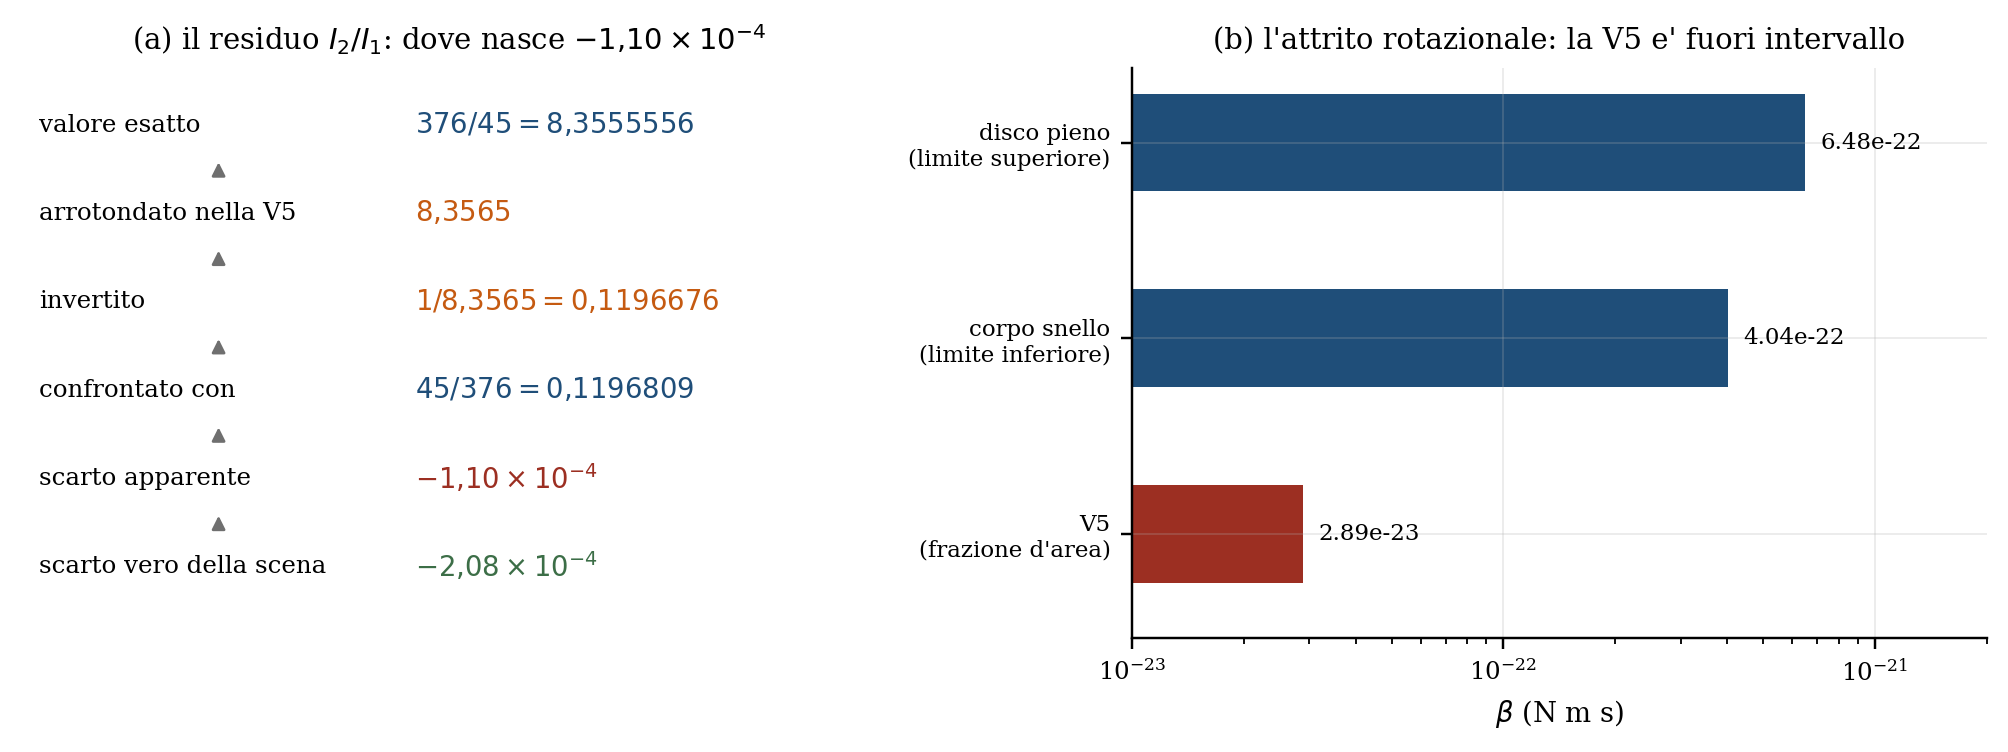
\includegraphics[width=\textwidth]{../figure/fig10_residui.png}
\caption{\textbf{(a)} La catena di valori che produce il numero della V5: nessuno dei
tre coincide, e il residuo vero \`e quello della scena ($-2{,}1\times10^{-4}$).
\textbf{(b)} L'attrito rotazionale: la stima della V5 (frazione di area bagnata) sta
sotto il limite inferiore dedotto dalla teoria dei corpi snelli, e dunque fuori
dall'intervallo fisicamente ammesso.}
\label{fig:residui}
\end{figure}

%=====================================================================
\section{Il modello unico}
%=====================================================================

La V5 usava tre definizioni di coppia in punti diversi del testo. La V6 ne usa una, e
la dichiara per quello che \`e: un limite.
\begin{equation}
\tau=(\ell+s)\,\frac{P_{\rm ass}}{\omega_{\rm ott}},
\qquad
F=\frac{I\,\sigma_{\rm pr}}{c},
\qquad
\omega_{\rm ott}=\frac{2\pi c}{\lambda},
\label{eq:modello}
\end{equation}
con $\ell$ momento angolare orbitale per fotone, $s=\pm1$ quello di polarizzazione,
$I=P/A_{\rm fascio}$ e $\sigma_{\rm pr}=\sigma_{\rm ext}-g\,\sigma_{\rm sca}$.

\subsection{Perch\'e sono due limiti}

La prima equazione dice: ogni fotone assorbito cede tutto il suo momento angolare
$(\ell+s)\hbar$. \`E vero solo se l'assorbimento \`e completo e se il momento angolare
non viene restituito al campo; per il nucleo di \SI{40}{nm} l'assorbimento \`e il
79\,\% dell'estinzione, quindi il limite \`e ragionevole ma non esatto. La seconda
dice: ogni fotone intercettato cede tutta la quantit\`a di moto assiale, e perde
validit\`a quando lo scattering \`e in avanti ($g\to1$).

Le due equazioni non vanno sommate: sono canali distinti, e il secondo non genera
coppia se il fascio \`e simmetrico. Il punto di metodo \`e che \emph{nessuna delle due
contiene il raggio}. Nel modello unico la coppia dipende dalla potenza assorbita e dal
momento angolare per fotone, non dalla dimensione del rotore. La geometria entra in
$\beta$ e in $I$, cio\`e nella risposta, non nella forzante.

\subsection{L'identit\`a che la V5 violava}

Da \eqref{eq:modello} e da $D_r=k_BT/\beta$ segue
\begin{equation}
Pe_r=\frac{\omega_{\rm ss}}{D_r}=\frac{\tau/\beta}{k_BT/\beta}=\frac{\tau}{k_BT},
\label{eq:identita}
\end{equation}
che non dipende da $\beta$. La V5 riportava due valori per la stessa grandezza,
$6{,}1\times10^{-4}$ e $8{,}8\times10^{-3}$, proprio perch\'e nel secondo calcolo
usava il $\beta$ del telaio e nel primo la diffusione della sfera equivalente.
L'identit\`a \eqref{eq:identita} \`e un test di coerenza che il codice esegue a ogni
esecuzione.

Poich\'e $P_{\rm ass}=\eta_{\rm ass}P$ e $P/\omega_{\rm ott}=\dot N\hbar$, si pu\`o
leggere \eqref{eq:identita} in forma pi\`u trasparente:
$Pe_r=(\ell+s)\,\dot N_{\rm ass}\hbar/k_BT$. La soglia $Pe_r=1$ \`e una condizione
sul \emph{tasso} di momento angolare: servono $k_BT/\hbar=4{,}1\times10^{13}$ quanti
al secondo, cio\`e \SI{15}{\micro W} di potenza assorbita con $\ell+s=1$, che alla
frazione assorbita di questa configurazione corrispondono a \SI{1.3}{mW} incidenti.

\begin{figure}[H]
\centering
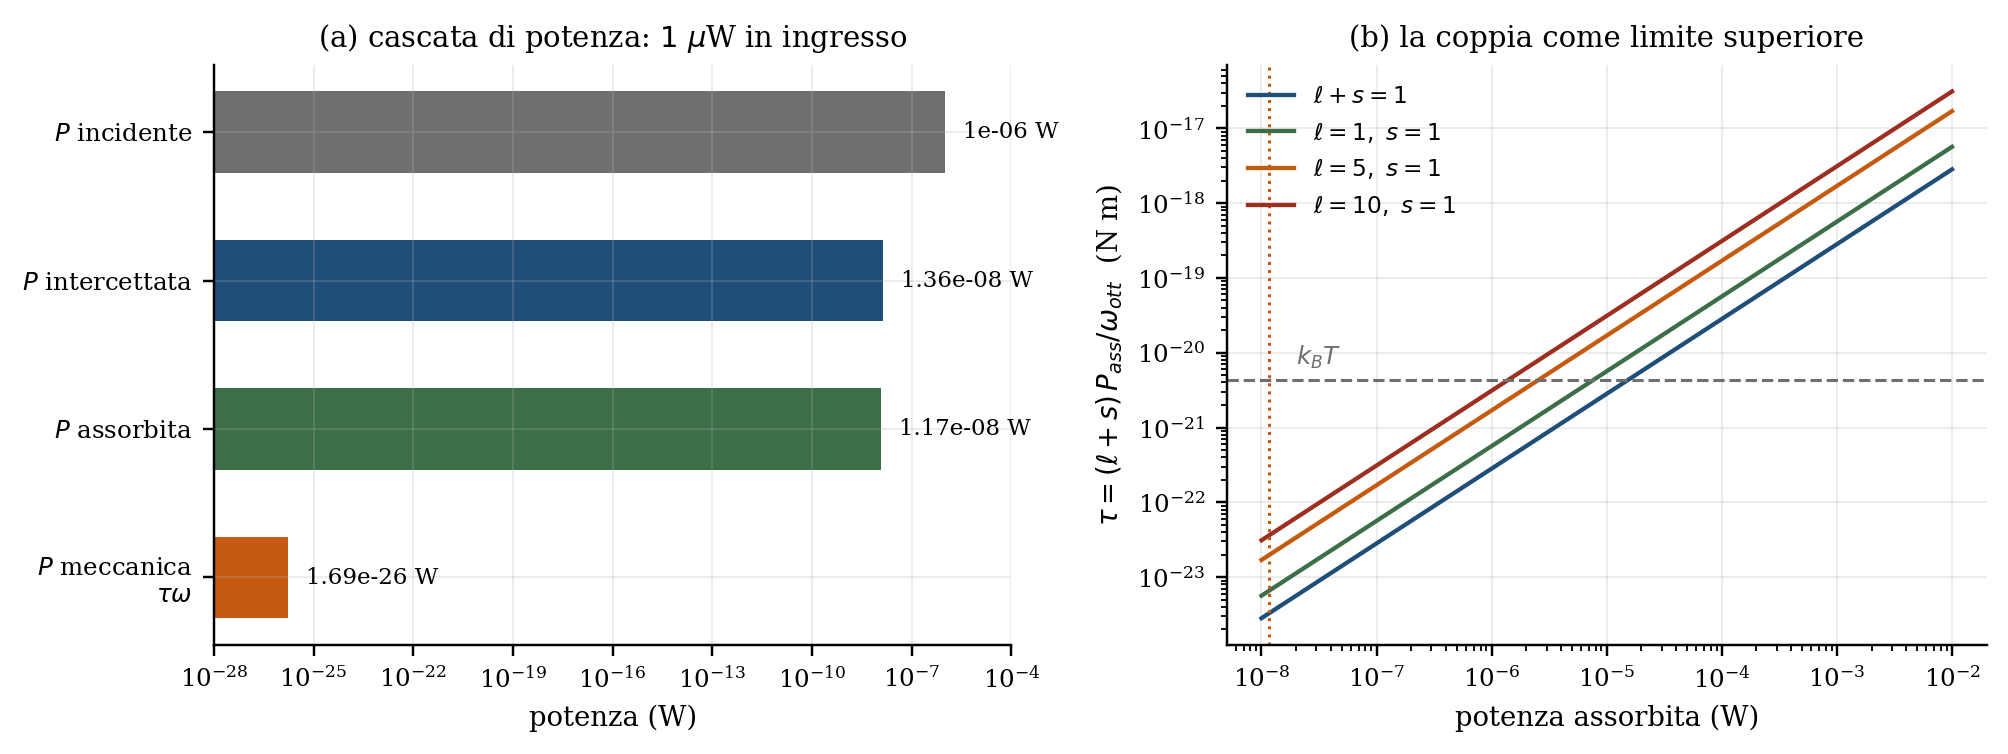
\includegraphics[width=\textwidth]{../figure/fig01_modello.png}
\caption{\textbf{(a)} La cascata di potenza a \SI{1}{\micro W} di ingresso:
l'$1{,}36$\,\% intercettato, l'$86$\,\% di questo assorbito, e la potenza meccanica
estratta, $1{,}7\times10^{-26}$\,W. \textbf{(b)} La coppia \eqref{eq:modello} contro
la potenza assorbita per quattro valori di $\ell+s$; la linea tratteggiata \`e $k_BT$.}
\label{fig:modello}
\end{figure}

\begin{table}[H]
\centering\small
\caption{Bilancio a \SI{1}{\micro W} incidente, $w_0=\SI{500}{nm}$.}
\label{tab:potenza}
\begin{tabular}{lrl}
\toprule
Grandezza & Valore & nota \\
\midrule
$P_{\rm inc}$ & \SI{1}{\micro W} & potenza di riferimento \\
$P_{\rm int}=I\sigma_{\rm pr}$ & \SI{13.56}{nW} & $1{,}356$\,\% del fascio \\
$P_{\rm abs}=I\sigma_{\rm abs}$ & \SI{11.70}{nW} & $86{,}3$\,\% dell'intercettato \\
$P_{\rm sca}$ & \SI{1.85}{nW} & portato via senza coppia \\
$\tau=(\ell+s)P_{\rm abs}/\omega_{\rm ott}$ & $3{,}305\times10^{-24}$\,N\,m & V5: $2{,}610$ \\
$P_{\rm mecc}=\tau\omega_{\rm ss}$ & $1{,}7\times10^{-26}$\,W & efficienza $1{,}4\times10^{-18}$ \\
\bottomrule
\end{tabular}
\end{table}

L'ultima riga \`e la pi\`u severa. Il rapporto fra potenza meccanica estratta e
potenza assorbita \`e $1{,}4\times10^{-18}$: il dispositivo non \`e una macchina che
converte luce in rotazione, \`e una resistenza che scalda. Non dipende dalla geometria
n\'e dal modello di coppia, ma dal fatto che $\omega_{\rm ss}\ll\omega_{\rm ott}$: i
fotoni sono $10^{15}$ volte pi\`u ``veloci'' del rotore. Un rotore ottico pu\`o essere
un sensore di coppia eccellente, e lo \`e: non pu\`o essere un attuatore.

%=====================================================================
\section{Audit ottico}
\label{sec:ottica}
%=====================================================================

\subsection{Il raggio dei fili, e perch\'e cambia tutto}

La V5 dichiarava ``diametro 6,4 nm'' per i fili delle orbite e poi calcolava il
parametro di dimensione con $a=\SI{1.25}{nm}$. In regime di Rayleigh la sezione di un
cilindro \`e proporzionale ad $a^2$, quindi l'errore valeva un fattore 6,5 sulle
orbite, 36 sull'anello di bordo e 13 sulle lenti. Rifatto il conto con i raggi della
scena --- 3,2, 7,5 e 4,5 nm --- il contributo dei fili passa dal 3\,\% al 34\,\% della
sezione totale, la massa da $2{,}78$ a $8{,}21\times10^{-18}$\,kg e il momento
d'inerzia da $3{,}1\times10^{-32}$ a $4{,}6\times10^{-31}$\,kg\,m$^2$. Sono le
differenze fra Tabella~\ref{tab:confronto} e Tabella~\ref{tab:residui}. Nessun'altra
parte del modello ottico cambia: la forma delle righe non era sbagliata, la geometria
s\`i.

\subsection{Modelli usati e loro stato}

\begin{table}[H]
\centering\small
\caption{Stato dei modelli ottici. ``Esatto'' significa soluzione delle equazioni di
Maxwell per quella geometria; ``verificato'' confrontato con il proprio limite
analitico.}
\label{tab:ottica}
\begin{tabular}{p{3.4cm}p{3.0cm}p{2.8cm}p{4.6cm}}
\toprule
Elemento & modello & stato & verifica \\
\midrule
Nucleo \SI{40}{nm} & Mie esatta & esatto & $Q_{\rm ext}\ge Q_{\rm sca}$ su tutto il range \\
Fili 6,4/15/9\,nm & serie cilindrica $n\ge1$ & esatto a $<1$\,\% & contro Rayleigh: $0{,}3$\,\% a $x=0{,}038$ \\
Filo, limite & Rayleigh cilindrico & analitico & usato per $x<0{,}05$ \\
Guscio di ossido & Maxwell-Garnett quasi-statico & approssimato & limiti $f\to0,1$ esatti \\
$\varepsilon(a)$ & Drude con $\gamma=\gamma_b+Av_F/a$ & approssimato & confronto con bulk \\
Assemblaggio & somma incoerente & \emph{ipotesi} & limite coerente $N^2\sigma_1$ dichiarato \\
\bottomrule
\end{tabular}
\end{table}

Il termine $n=0$ delle formule cilindriche di Bohren-Huffman \`e instabile per
$x\to0$: a $x=0{,}015$ produce $Q_{\rm ext}=0{,}138$ al posto di $0{,}011$, un
artefatto della divergenza logaritmica di $H_0$. La serie della V6 parte da $n=1$ e
coincide con Rayleigh allo $0{,}3$\,\%. Un implementatore che si fosse fidato della
``formula completa'' avrebbe sovrastimato la coppia di un fattore 13.

\subsection{Dipendenza dalla dimensione e ossidazione}

La correzione di Drude $\gamma(a)=\gamma_{\rm bulk}+Av_F/a$ ($v_F=1{,}57\times10^6$\,m/s,
$\tau_{\rm bulk}=\SI{27}{fs}$) cambia $Q_{\rm abs}$ dell'$1{,}4$\,\% a \SI{40}{nm},
del $5$\,\% a \SI{10}{nm} e del $21$\,\% a \SI{2}{nm}: a \SI{532}{nm} il rame \`e
dominato dalle transizioni interbanda, non dal termine di Drude, e nel verde si
comporta meglio dell'oro e dell'argento.

Un guscio di Cu$_2$O cambia l'assorbimento in modo monotono: $+7{,}8$\,\% per
\SI{0.7}{nm}, $+15{,}8$\,\% per \SI{1.4}{nm}, $+51$\,\% per \SI{5.4}{nm}, saturando
oltre gli \SI{8}{nm}. L'effetto \`e nella direzione ``pi\`u coppia'', ma va letto con
la termica: lo stesso ossido alza l'emissivit\`a e abbassa la temperatura di regime.
In vuoto l'ossidazione \`e un vantaggio termico prima che ottico.

L'incertezza dominante non \`e per\`o n\'e $\varepsilon(a)$ n\'e l'ossido, ma la
dispersione dei dati ottici: $\pm30$\,\% su $k$ sposta $\sigma_{\rm pr}$ di
$-39/+44$\,\% e $\sigma_{\rm abs}$ di $-47/+60$\,\%, mentre la stessa variazione su
$n$ vale $-10/+6$\,\%. Chi misura questa struttura deve prima fissare $k$.

\subsection{L'assemblaggio, e ci\`o che manca}

La sezione del telaio \`e la somma incoerente delle sezioni dei singoli elementi: \`e
un'ipotesi, valida se la distanza fra i diffusori supera la lunghezza di coerenza
laterale del fascio e se l'accoppiamento di campo vicino \`e debole. A \SI{250}{nm} di
distanza e $kD=3$ l'ipotesi \`e ragionevole ma non dimostrata; il limite superiore
rigoroso \`e $N^2\sigma_1$, un fattore 4 sopra. Una verifica DDA/FDTD dell'intero
telaio resta aperta, ed \`e il solo punto della V6 in cui un calcolo esterno pu\`o
cambiare un numero del testo.

\begin{figure}[H]
\centering
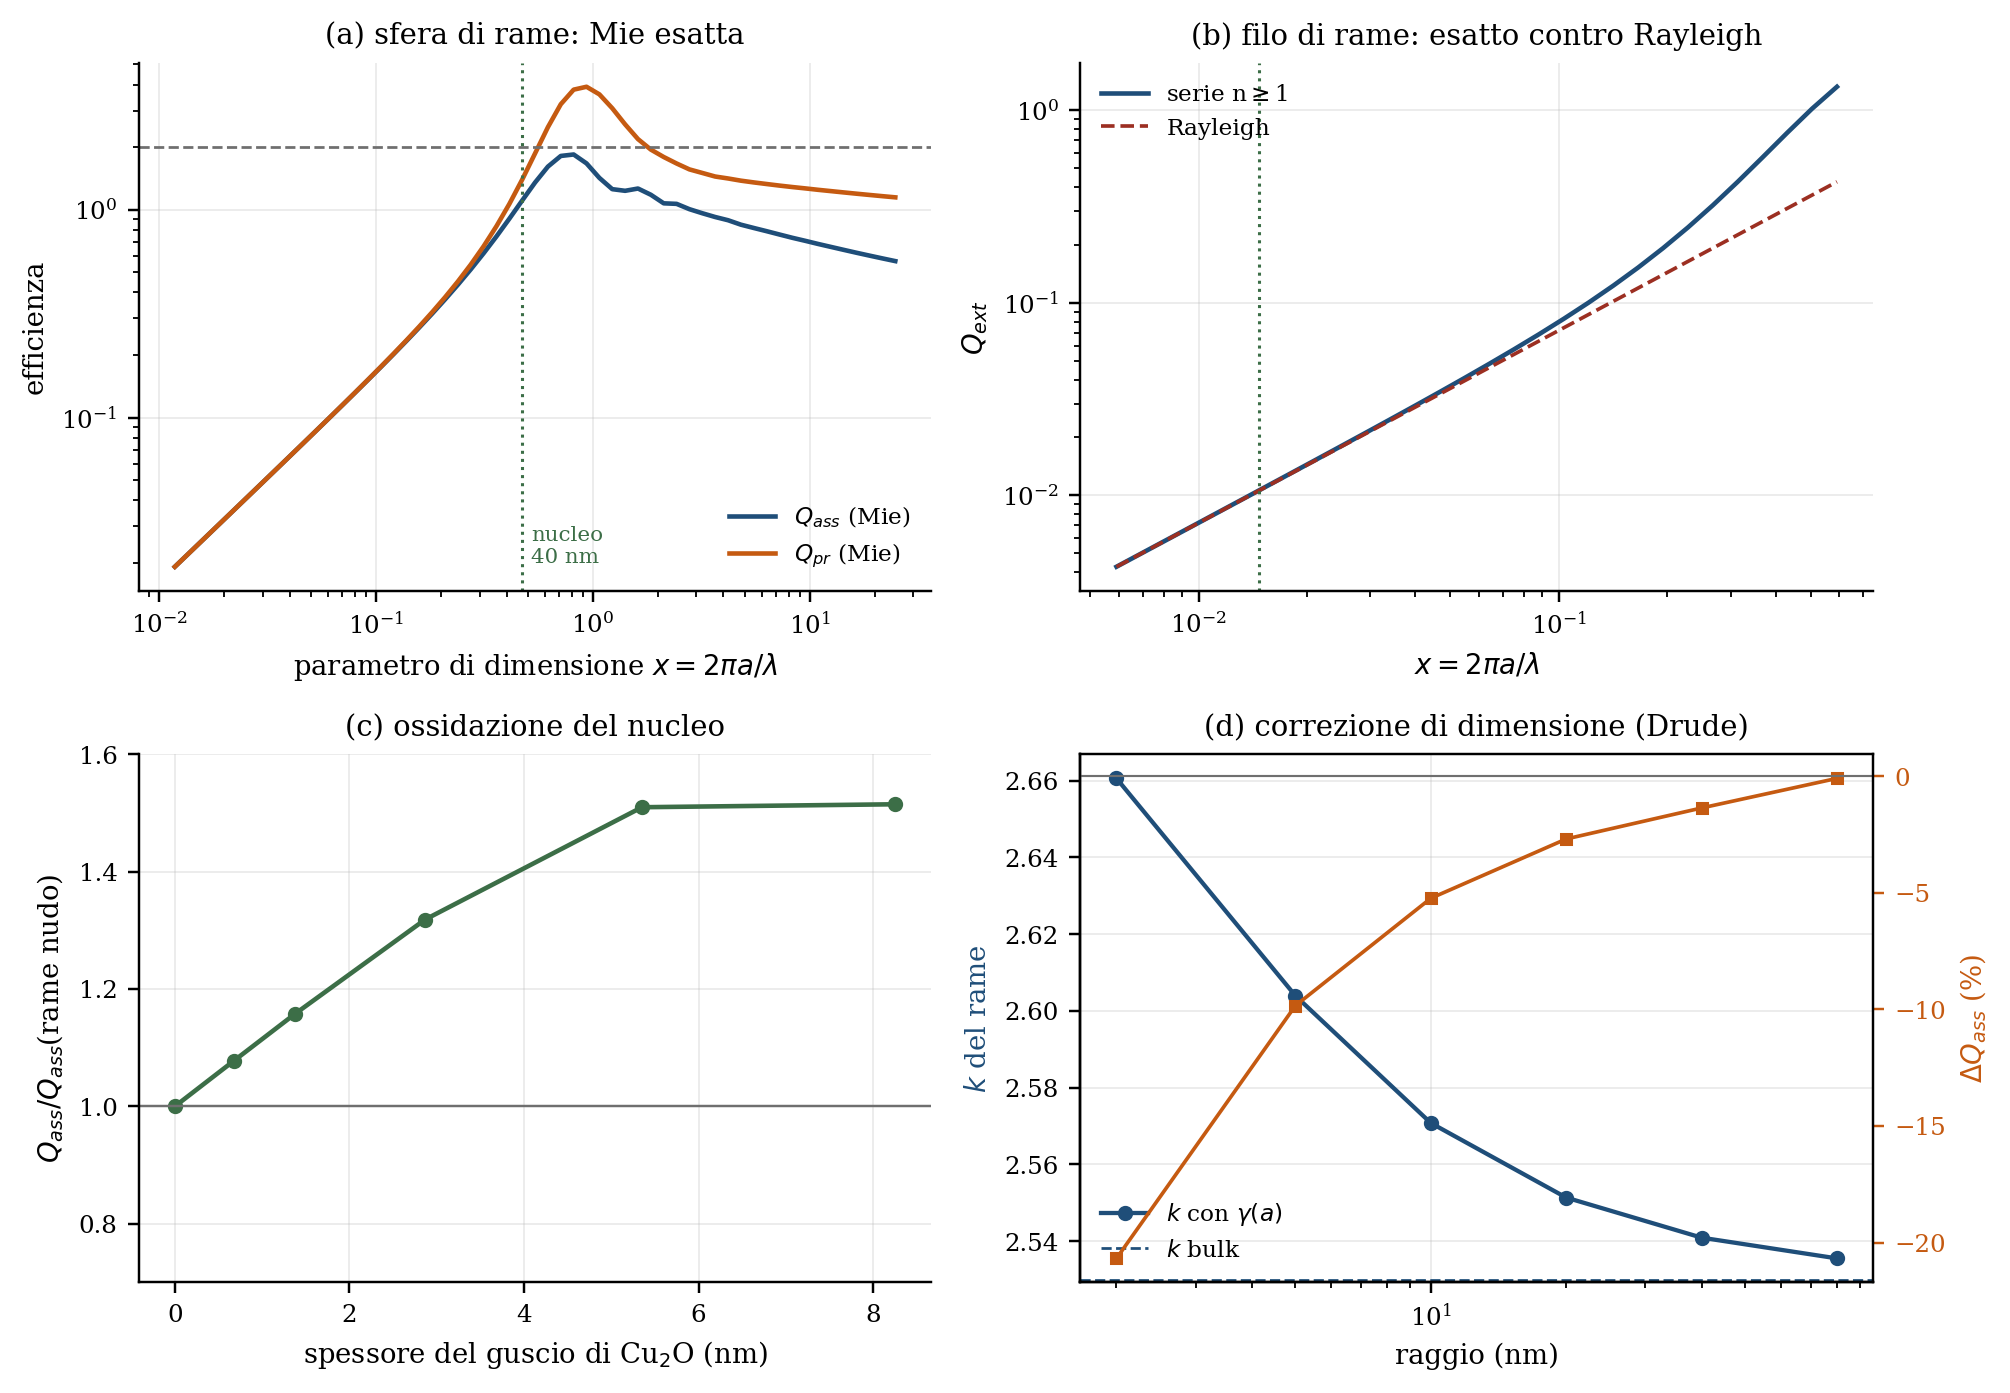
\includegraphics[width=\textwidth]{../figure/fig02_ottica.png}
\caption{\textbf{(a)} Efficienze di Mie per una sfera di rame: il nucleo di
\SI{40}{nm} sta a $x=0{,}47$, dove $Q_{\rm pr}=1{,}40$ e $Q_{\rm abs}=1{,}11$.
\textbf{(b)} La serie cilindrica contro il limite di Rayleigh: coincidono fino a
$x\approx0{,}05$; i fili stanno nella zona di accordo. \textbf{(c)} Effetto di un
guscio di Cu$_2$O. \textbf{(d)} Correzione di Drude: $k$ cresce al diminuire del
raggio, ma a \SI{40}{nm} l'effetto su $Q_{\rm abs}$ \`e dell'$1{,}4$\,\%.}
\label{fig:ottica}
\end{figure}

%=====================================================================
\section{Bilancio termico}
\label{sec:termica}
%=====================================================================

Il bilancio che mancava si scrive in una riga,
$P_{\rm ass}=P_{\rm diss}+P_{\rm out}$, e si chiude subito:
$P_{\rm diss}=\beta\omega_{\rm ss}^2=1{,}7\times10^{-26}$\,W, cio\`e $10^{-18}$ della
potenza assorbita. In regime stazionario \emph{tutta} la potenza assorbita esce come
calore, e i due percorsi sono la conduzione nel mezzo e l'irraggiamento.

Nel fluido, con numero di Nusselt unitario (a queste scale $Ra\sim10^{-18}$):
\begin{equation}
\Delta T_{\rm fluido}=\frac{P_{\rm ass}}{4\pi\kappa_m r}=\SI{0.026}{K}
\quad\text{a \SI{1}{\micro W}.}
\end{equation}
La soglia di ebollizione locale arriva a \SI{3.9}{mW}. In acqua il problema termico
non esiste.

In vuoto comanda, e il punto delicato \`e l'area. La superficie metallica esposta
\`e $A=2\pi\sum a_iL_i+4\pi r_{\rm core}^2=2{,}69\times10^{-13}$\,m$^2$, sei volte
meno dell'inviluppo sferico $4\pi R_{\rm out}^2$ usato nella 6.0:
\begin{equation}
T=\left(T_0^4+\frac{P_{\rm ass}}{\epsilon\sigma_{\rm SB}A}\right)^{1/4}.
\end{equation}
A \SI{1}{\micro W} si ottiene \SI{2250}{K} con $\epsilon=0{,}03$ e \SI{1505}{K} con
$\epsilon=0{,}15$: in entrambi i casi il rotore ha superato la fusione del rame
(\SI{1358}{K}). La potenza incidente che porta a fusione \`e
\SI{0.132}{\micro W} e \SI{0.662}{\micro W}; il tempo adiabatico di fusione \`e
\SI{0.28}{ms}, contro uno spin-up in vuoto che richiede \SI{24}{s}
(Tabella~\ref{tab:regimi}). \`E il risultato pi\`u solido della revisione: in vuoto il
collo di bottiglia non \`e la coppia, \`e la temperatura, e non \`e negoziabile con la
geometria.

Sull'emissivit\`a conviene essere espliciti, perch\'e la 6.0 usava $\epsilon=0{,}6$.
L'emissivit\`a di un oggetto sub-lunghezza d'onda dipende dall'assorbimento
volumetrico a \SI{10}{\micro m}, non dalla costante ottica massiva di un ossido
sottile: un guscio di \SI{1.4}{nm} di Cu$_2$O non porta l'oggetto a
$\epsilon=0{,}6$. La V6 usa un intervallo $0{,}03$--$0{,}15$ e mostra che nemmeno
l'estremo superiore salva il rotore.

\begin{table}[H]
\centering\small
\caption{Bilancio termico della configurazione di riferimento. $P_{\rm fus}$ \`e la
potenza \emph{assorbita} che porta a fusione ($1{,}55$ e $7{,}75$\,nW), cio\`e
\SI{0.13}{}--\SI{0.66}{\micro W} incidenti con $\eta_{\rm abs}=1{,}17$\,\%.}
\label{tab:termica}
\begin{tabular}{rrrrrr}
\toprule
$P_{\rm inc}$ & $P_{\rm abs}$ & $\Delta T$ acqua & $T$ vuoto ($\epsilon=0{,}03$) & $T$ vuoto ($\epsilon=0{,}15$) & $t_{\rm ad}$ \\
\midrule
\SI{1}{\micro W} & \SI{11.7}{nW} & \SI{0.026}{K} & \SI{2250}{K} & \SI{1505}{K} & \SI{0.28}{ms} \\
\SI{100}{\micro W} & \SI{1.17}{\micro W} & \SI{2.6}{K} & \SI{7113}{K} & \SI{4757}{K} & \SI{2.8}{\micro s} \\
\SI{10}{mW} & \SI{117}{\micro W} & \SI{258}{K} & \SI{22495}{K} & \SI{15043}{K} & \SI{28}{ns} \\
\bottomrule
\end{tabular}
\end{table}

Due conseguenze operative. Primo: in vuoto l'emissivit\`a \`e una variabile di
progetto di primo ordine, pi\`u della geometria. Secondo: la pulsata, che la V5
trattava come regime dinamico, \`e l'unico modo di stare in vuoto ad alta potenza; il
duty cycle \`e $P_{\rm fus}/P_{\rm abs}$ alla potenza di picco.

\begin{figure}[H]
\centering
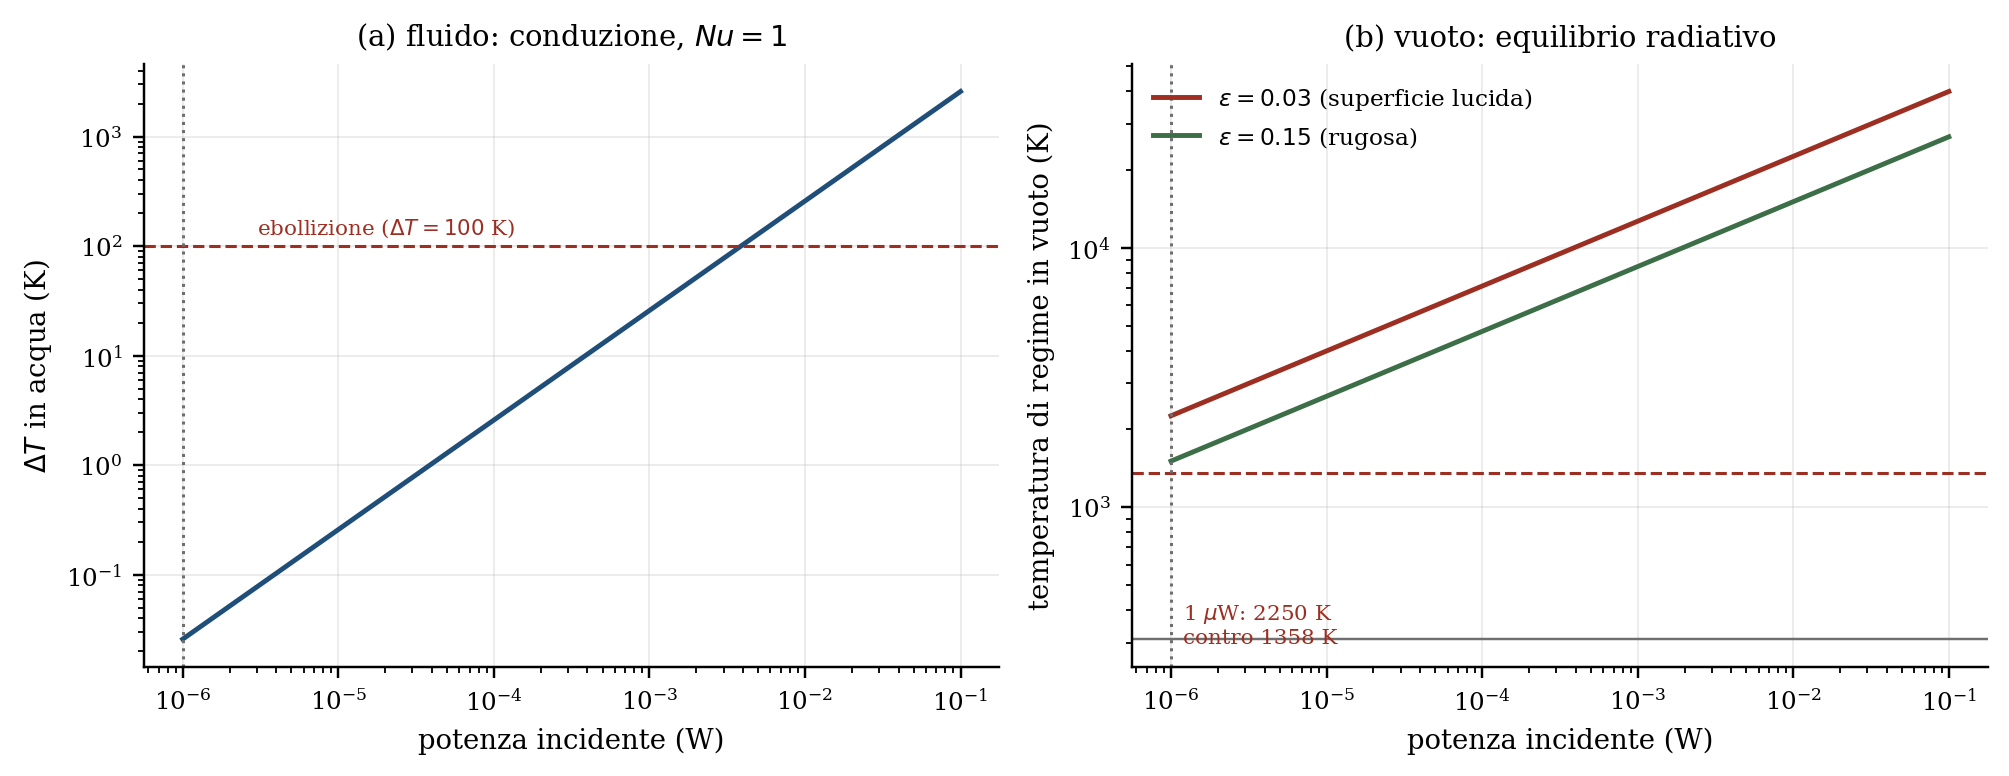
\includegraphics[width=\textwidth]{../figure/fig03_termica.png}
\caption{\textbf{(a)} Riscaldamento in acqua: \SI{0.026}{K} a \SI{1}{\micro W},
ebollizione a \SI{3.9}{mW}. \textbf{(b)} Equilibrio radiativo con la superficie
metallica reale: a \SI{1}{\micro W} entrambe le emissivit\`a superano la fusione.}
\label{fig:termica}
\end{figure}

%=====================================================================
\section{Baseline a pari massa}
\label{sec:baseline}
%=====================================================================

Questa \`e la sezione che risponde alla domanda ``che cosa aggiungono le lenti e il
Contro-spin''. Il confronto \`e a massa costante ($8{,}211\times10^{-18}$\,kg), a
potenza costante (\SI{1}{\micro W}), a lunghezza d'onda e mezzo costanti.

\begin{table}[H]
\centering\footnotesize
\setlength{\tabcolsep}{3.5pt}
\caption{Sei geometrie a pari massa ($8{,}211\times10^{-18}$\,kg), $P=\SI{1}{\micro W}$,
$w_0=\SI{500}{nm}$. $\sigma_{ass}$ \`e la sezione usata: per il reticolo \`e il calcolo
per elemento, per le altre la sfera di pari volume; $Pe_r$ e $\omega_{ss}$ riportano
l'intervallo ottico dichiarato nel testo. $t_r$ \`e il tempo di rottura in vuoto.}
\label{tab:baseline}
\begin{tabular}{lrrrrrrr}
\hline
Geometria & $R$ (nm) & $\beta$ (N\,m\,s) & $\sigma_{ass}$ (m$^2$) & $\tau$ (N\,m) & $Pe_r$ & $\omega_{ss}$ (rad/s) & $t_{r}$ (s) \\
\hline
Reticolo (V5) & 370 & $4{,}04$--$6{,}48\times10^{-22}$ & $9{,}19\times10^{-15}$ & $3{,}31\times10^{-24}$ & $7{,}72\times10^{-4}$ & $5{,}10$--$8{,}19\times10^{-3}$ & $56{,}4$ \\
Disco pieno & 143 & $3{,}73\times10^{-23}$ & $2{,}07\times10^{-14}$ & $7{,}44\times10^{-24}$ & $1{,}74$--$5{,}22\times10^{-3}$ & $0{,}199$--$0{,}598$ & $11{,}8$ \\
Anello & 420 & $7{,}21$--$9{,}51\times10^{-22}$ & $2{,}07\times10^{-14}$ & $7{,}44\times10^{-24}$ & $1{,}74$--$5{,}22\times10^{-3}$ & $7{,}83\times10^{-3}$--$0{,}031$ & $69{,}3$ \\
Sfera & 60 & $6{,}60\times10^{-24}$ & $2{,}07\times10^{-14}$ & $7{,}44\times10^{-24}$ & $1{,}74\times10^{-3}$ & $1{,}13$ & $3{,}97$ \\
Nanomanubrio & 143 & $2{,}64$--$3{,}30\times10^{-23}$ & $2{,}07\times10^{-14}$ & $7{,}44\times10^{-24}$ & $1{,}74$--$5{,}22\times10^{-3}$ & $0{,}226$--$0{,}846$ & $11{,}6$ \\
Silice anisotropa & 96 & $2{,}69\times10^{-23}$ & $1{,}01\times10^{-20}$ & $6{,}68\times10^{-27}$ & $1{,}56$--$4{,}68\times10^{-6}$ & $2{,}49$--$7{,}46\times10^{-4}$ & $7{,}1\times10^{3}$ \\
\hline
\end{tabular}

\end{table}

\begin{figure}[H]
\centering
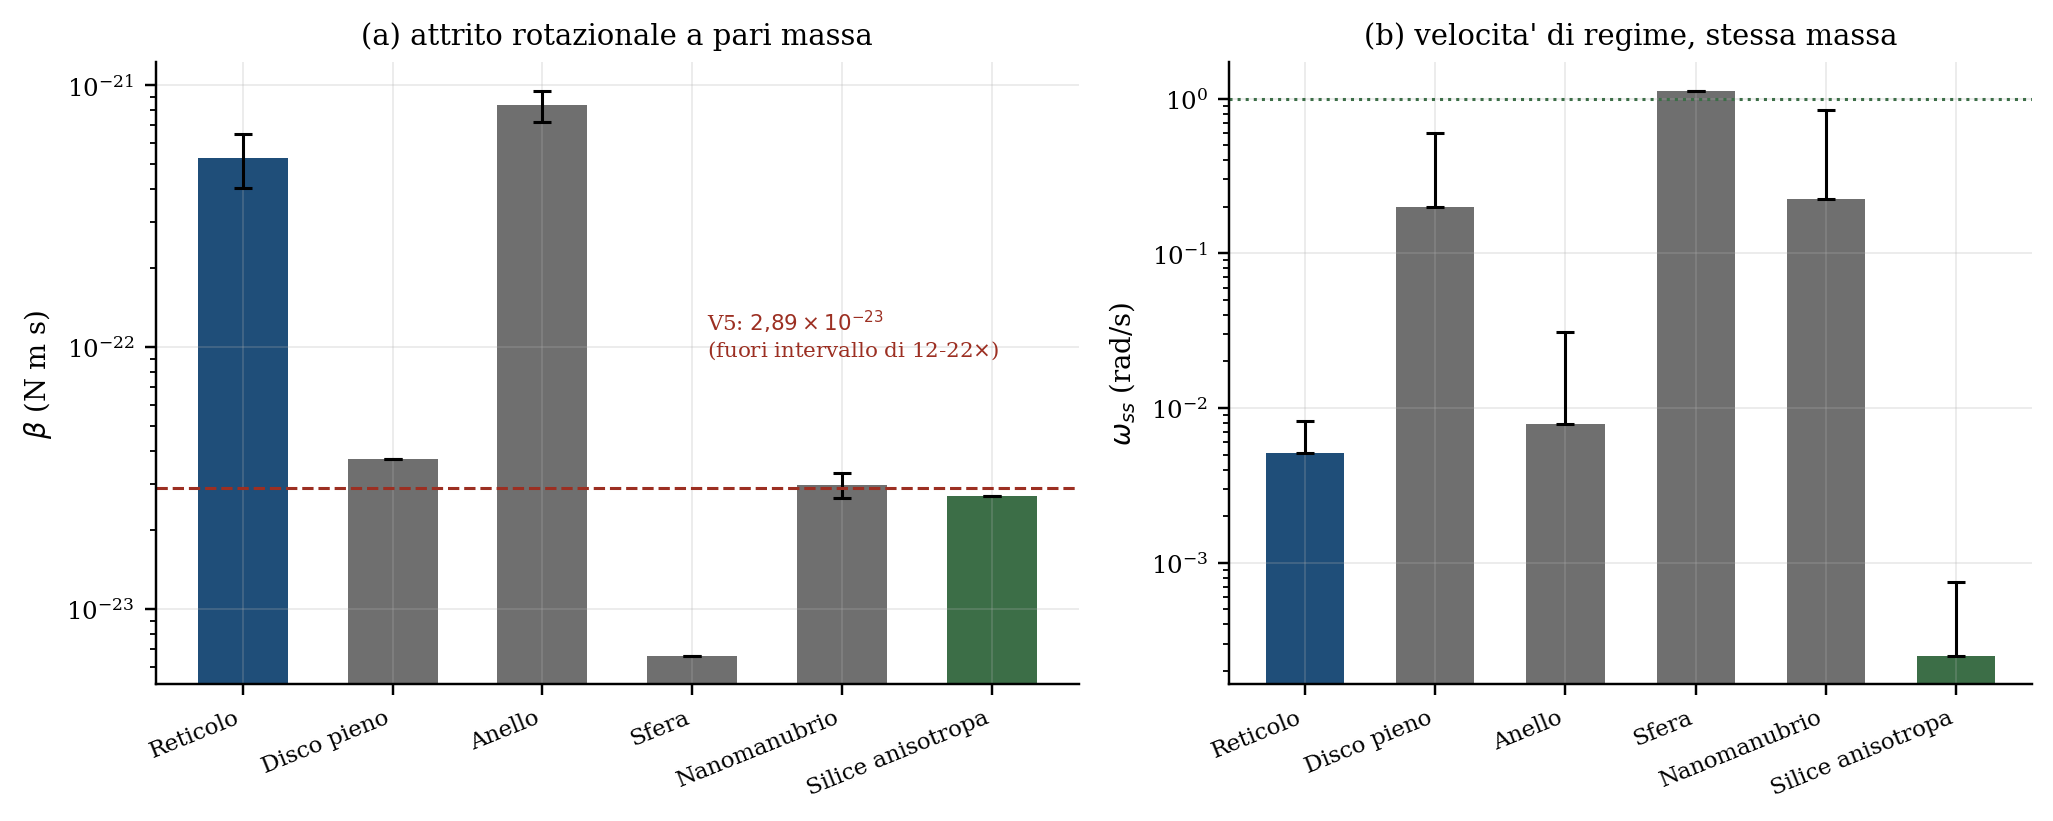
\includegraphics[width=\textwidth]{../figure/fig04_baseline.png}
\caption{\textbf{(a)} Attrito rotazionale delle sei geometrie, con l'intervallo
fisico per i corpi snelli; la linea rossa \`e la stima della V5. \textbf{(b)}
Velocit\`a di regime con la banda ottica dichiarata nel testo.}
\label{fig:baseline}
\end{figure}

\subsection{La coppia non \`e un risultato: \`e un'ipotesi dichiarata}

Nella 6.0 tutte le geometrie ricevevano la sezione della sfera di pari volume, e
$Pe_r$ risultava identico per costruzione. Era un'assunzione travestita da risultato,
e la 6.1 la corregge in due modi.

Primo, il reticolo usa la \emph{sua} sezione, calcolata elemento per elemento:
$\sigma_{\rm abs}=9{,}19\times10^{-15}$\,m$^2$, che corrisponde a
$Pe_r=7{,}72\times10^{-4}$. La sfera compatta di pari massa ($r=\SI{60}{nm}$) ne
assorbe $2{,}07\times10^{-14}$, il $125$\,\% in pi\`u, e d\`a $Pe_r=1{,}74\times10^{-3}$.
La differenza \`e fisica e si spiega in una riga: nel limite di Rayleigh
l'assorbimento \`e proporzionale al volume, ma il nucleo sta a $x=0{,}47$ e la sfera
equivalente a $x=0{,}71$, in una regione in cui $Q_{\rm abs}$ cresce con la
dimensione. Il reticolo, spalmando lo stesso materiale in fili sottili, perde il
guadagno di risonanza.

Secondo, per disco, anello e manubrio la sezione \`e data come \emph{banda}: da una a
tre volte il valore di pari volume, perch\'e le risonanze di forma a volume fissato
spostano $Q_{\rm abs}$ di un fattore 2--3 e una stima vera richiede un calcolo DDA per
forma. La Tabella~\ref{tab:baseline} riporta l'intervallo, e la conclusione ottica va
letta come condizionale: \emph{se} la sezione resta entro tre volte quella di volume,
allora a pari massa nessuna di queste geometrie guadagna pi\`u di un fattore 3 in
$Pe_r$.

Per l'attrito, invece, il risultato non \`e condizionale: $\beta$ va da
$6{,}6\times10^{-24}$ (sfera) a $8{,}4\times10^{-22}$ (anello), due decadi, ed \`e
calcolato per forma. \`E questa la parte che regge.

\subsection{Che cosa fanno i fili, le lenti e il Contro-spin}

La scomposizione del reticolo, con i raggi di filo corretti:
\begin{center}\small
\begin{tabular}{lrrr}
\toprule
componente & quota di massa & quota di $\sigma_{\rm abs}$ & quota di $\beta$ \\
\midrule
nucleo sferico \SI{40}{nm} & 29{,}3\,\% & 60{,}6\,\% & 0{,}5\,\% \\
telaio (orbite, bordo, lenti) & 70{,}7\,\% & 39{,}4\,\% & 99{,}5\,\% \\
\bottomrule
\end{tabular}
\end{center}
Con i raggi di filo della scena il telaio non \`e pi\`u otticamente marginale: porta il
39\,\% della coppia. Resta per\`o un moltiplicatore di attrito di 209 rispetto al solo
nucleo. Se il suo ruolo fosse ottico sarebbe un compromesso; se il ruolo \`e
meccanico --- tenere il nucleo in asse, distribuire la massa, definire il momento
d'inerzia --- va giudicato su quello, e la V6 non trova nessuna misura che lo
giustifichi a questa scala.

Il Contro-spin va in appendice con il 45/376. Qui basta la conseguenza quantitativa:
aggiunge momento d'inerzia e attrito senza aggiungere coppia. Mantenere il rapporto
richiede un vincolo meccanico, e un vincolo meccanico fra due rotori li rende un corpo
rigido unico.

\subsection{La struttura alternativa}

Due varianti emergono. Il \emph{disco pieno} a pari massa ($R=\SI{143}{nm}$,
$t=\SI{14}{nm}$) ha $\omega_{\rm ss}$ 39 volte maggiore del reticolo e nessun elemento
otticamente inutile. La \emph{silice anisotropa} \`e l'unica geometria che cambia il
canale fisico: non assorbe ($\sigma_{\rm abs}=1{,}0\times10^{-20}$\,m$^2$) e lavora
per ritardo di fase, $\tau=(P_{\rm int}/\omega_{\rm ott})\sin^2(\delta/2)$; a
\SI{1}{\micro W} in acqua vale $6{,}7\times10^{-27}$\,N\,m, quattrocento volte meno
del rame; in vuoto ad alta potenza \`e l'unica che non fonde. La conclusione non \`e
che il rame sia meglio: \`e che \emph{il canale di coppia va scelto insieme al mezzo},
e la V6 lo mostra invece di assumerlo.

\begin{figure}[H]
\centering
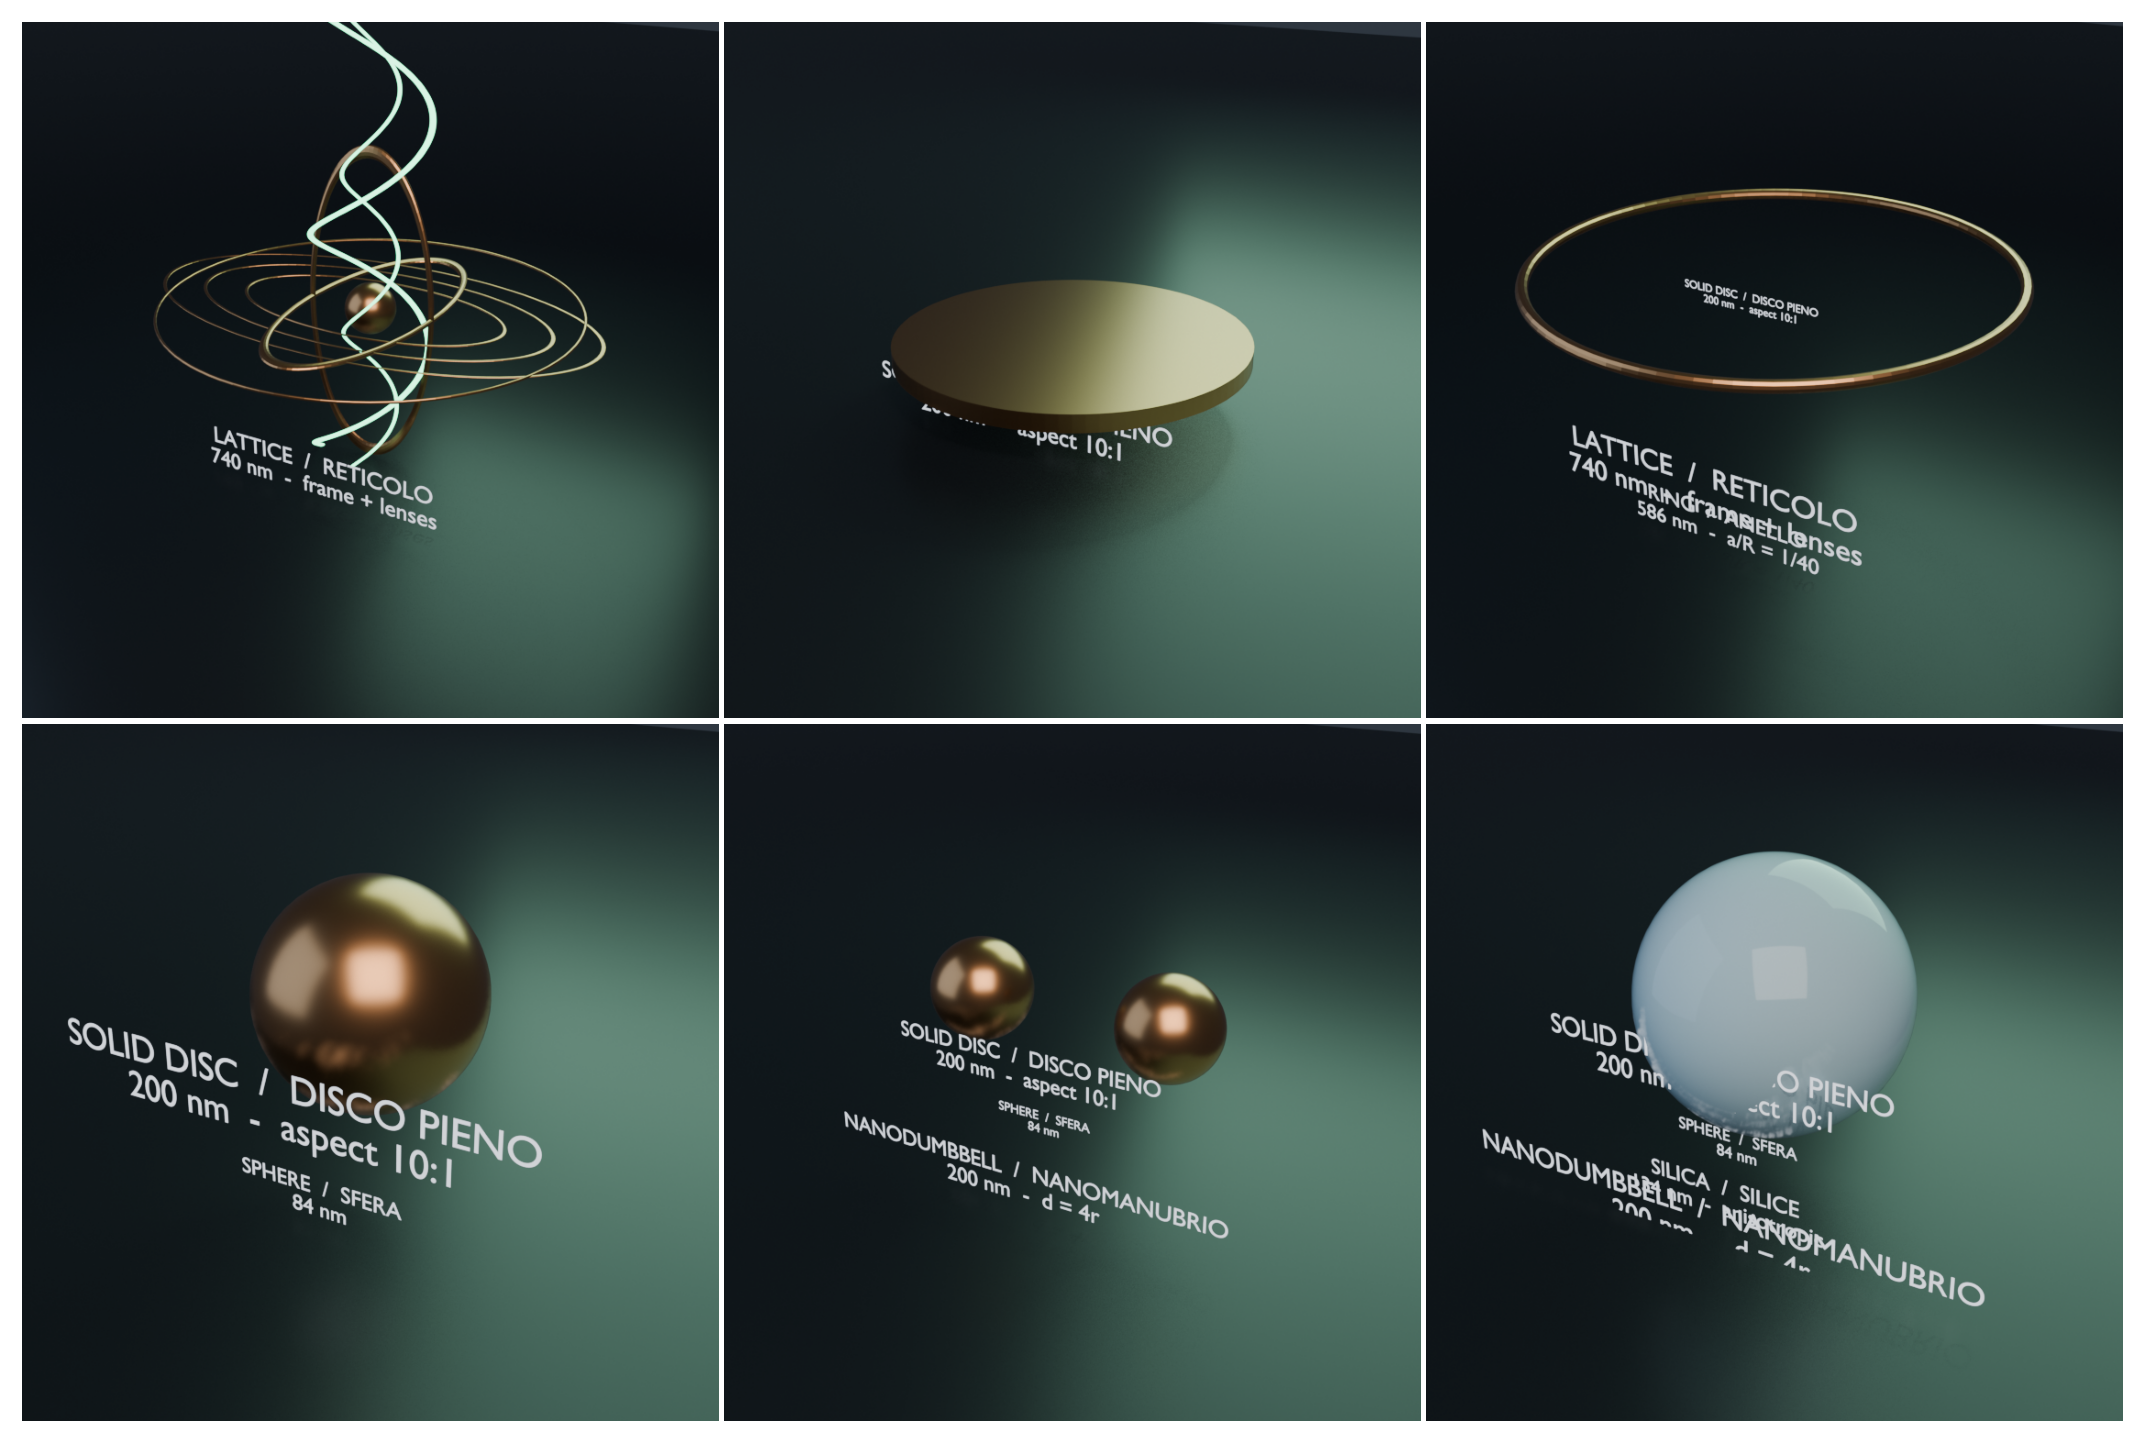
\includegraphics[width=\textwidth]{../figure/fig11_baseline_render.png}
\caption{Le sei geometrie a pari massa, renderizzate con lo stesso ingombro in
immagine (la dimensione reale \`e nella didascalia di ciascun riquadro). La
differenza di scala \`e il punto: la stessa massa, distribuita in un telaio di
\SI{740}{nm} o in una sfera di \SI{84}{nm}, cambia $\beta$ di due decadi e $Pe_r$ di
un fattore 2.}
\label{fig:render_baseline}
\end{figure}

%=====================================================================
\section{Matrice dei regimi}
\label{sec:regimi}
%=====================================================================

La matrice incrocia quattro dimensioni esterne con due mezzi. Il fattore di scala \`e
$s=L/2R_{\rm out}$, quindi la colonna ``240 nm'' descrive un telaio ridotto, non la
configurazione di riferimento.

\begin{table}[H]
\centering\footnotesize
\setlength{\tabcolsep}{3.5pt}
\caption{Matrice dei regimi: quattro dimensioni esterne $L$ e due mezzi, $P=\SI{1}{\micro W}$.
In vuoto non esiste $\omega_{ss}$ (``--'') e il tempo di rottura prende il suo posto.
$T$ \`e la temperatura di regime con $\epsilon=0{,}15$; a \SI{1}{\micro W} supera
gi\`a la fusione del rame.}
\label{tab:regimi}
\begin{tabular}{llrrrrrrl}
\hline
$L$ & mezzo & $\eta_{int}$ & $\tau$ (N\,m) & $\omega$ (rad/s) & $Pe_r$ & $t_{rott}$ (s) & $T$ (K) & validit\`a \\
\hline
1 nm & fluido & $9{,}90\times10^{-8}$ & $2{,}41\times10^{-29}$ & $1{,}89$--$3{,}03$ & $5{,}64\times10^{-9}$ & -- & 310 & fuori dominio \\
1 nm & vuoto & $9{,}90\times10^{-8}$ & $2{,}41\times10^{-29}$ & -- & $5{,}64\times10^{-9}$ & $4{,}1\times10^{-4}$ & 1505 & fuori dominio \\
240 nm & fluido & $5{,}70\times10^{-3}$ & $1{,}39\times10^{-24}$ & $7{,}86\times10^{-3}$--$0{,}0126$ & $3{,}25\times10^{-4}$ & -- & 310 & valido \\
240 nm & vuoto & $5{,}70\times10^{-3}$ & $1{,}39\times10^{-24}$ & -- & $3{,}25\times10^{-4}$ & $23{,}7$ & 1505 & valido \\
1 $\mu$m & fluido & $0{,}099$ & $2{,}41\times10^{-23}$ & $1{,}89$--$3{,}03\times10^{-3}$ & $5{,}64\times10^{-3}$ & -- & 310 & valido \\
1 $\mu$m & vuoto & $0{,}099$ & $2{,}41\times10^{-23}$ & -- & $5{,}64\times10^{-3}$ & $412$ & 1505 & valido \\
1 m & fluido & $1$ & $2{,}82\times10^{-22}$ & $2{,}21\times10^{-20}$ & $0{,}066$ & -- & 310 & valido \\
1 m & vuoto & $1$ & $2{,}82\times10^{-22}$ & -- & $0{,}066$ & $3{,}5\times10^{25}$ & 310 & estrap. \\
\hline
\end{tabular}

\end{table}

\begin{figure}[H]
\centering
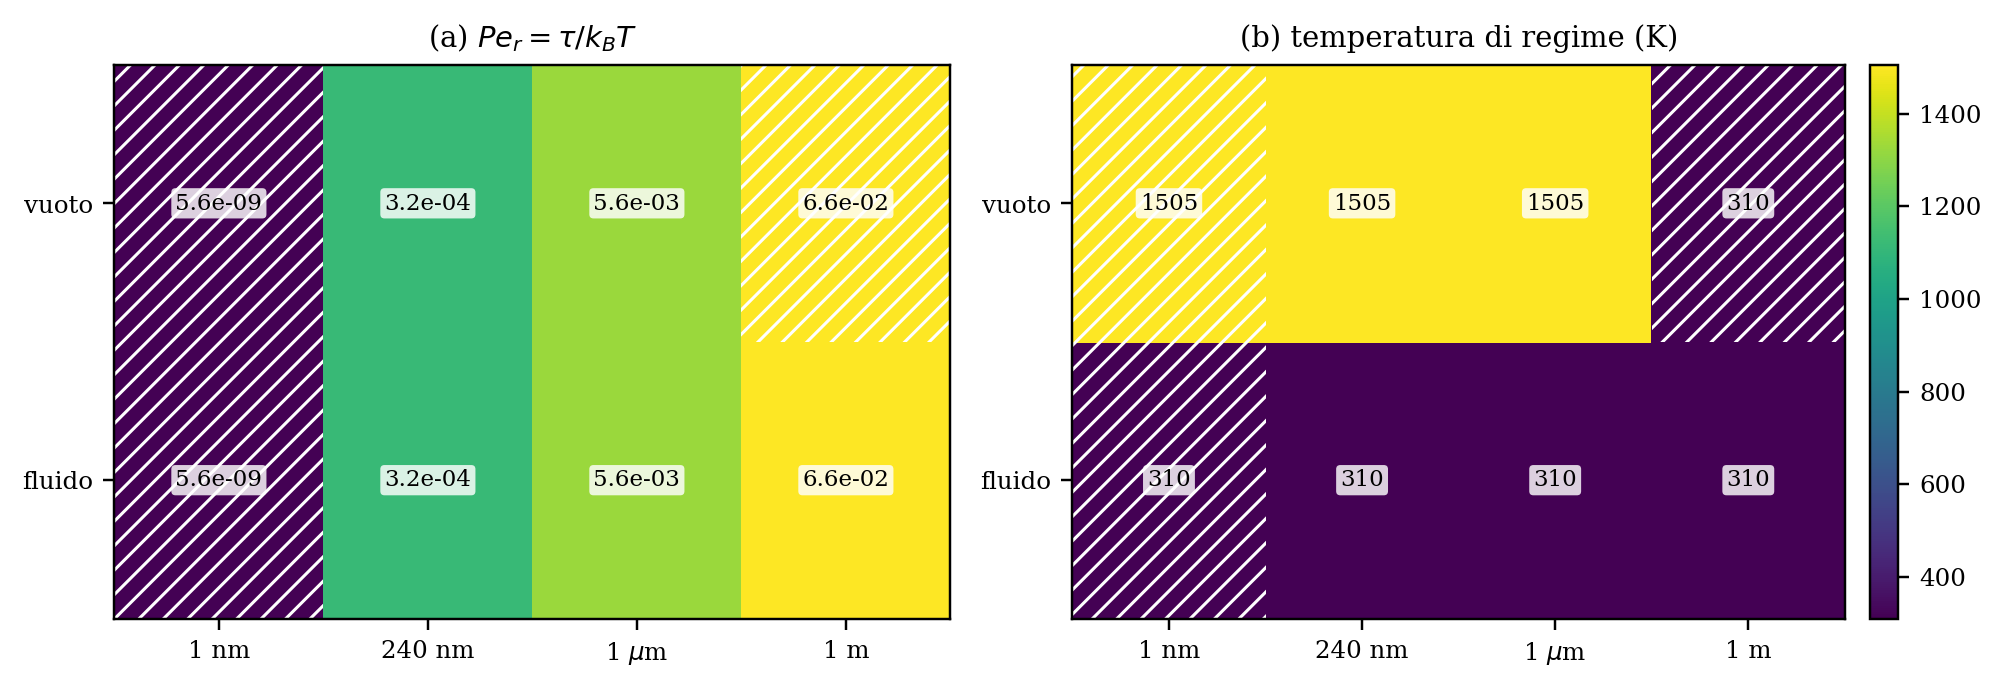
\includegraphics[width=\textwidth]{../figure/fig05_regimi.png}
\caption{Matrice dei regimi: $Pe_r$ e temperatura di regime. Le celle tratteggiate
sono fuori dal dominio di validit\`a (filo subatomico a \SI{1}{nm}, estrapolazione a
\SI{1}{m}). In vuoto $\omega_{\rm ss}$ non esiste: la casella riporta ``--'' e il
tempo di rottura prende il suo posto.}
\label{fig:regimi}
\end{figure}

Tre letture.

\textbf{Scala.} $Pe_r\propto\sigma_{\rm abs}\propto L^2$ finch\'e la struttura \`e
pi\`u piccola del fascio, poi satura a $P/(\omega_{\rm ott}k_BT)=0{,}066$. Non c'\`e
una scala privilegiata per la coppia: la geometria grande non guadagna in $Pe_r$,
perde in $\beta$.

\textbf{Mezzo.} In fluido esiste uno stato stazionario; in vuoto no. In vuoto la
grandezza che conta \`e il tempo di rottura, $t_r=I\omega_{\rm lim}/\tau$:
\SI{24}{s} a \SI{240}{nm}, \SI{410}{s} a \SI{1}{\micro m}. La temperatura, invece,
non dipende dalla scala in regime di Rayleigh ($P_{\rm ass}\propto R^2$ e
$A\propto R^2$): resta \SI{1505}{K} a ogni dimensione finch\'e l'intercettazione non
satura. Rimpicciolire il rotore non lo raffredda.

\textbf{Validit\`a.} Le due colonne estreme non sono fisica. A \SI{1}{nm} il filo
avrebbe un raggio di \SI{8.6}{pm}, meno di un atomo di rame (\SI{0.13}{nm}), e il
continuo non si applica; a \SI{1}{m} cambiano Reynolds e gravit\`a. La V6 le marca
invece di presentarle come ``invarianza su nove ordini di grandezza'':
l'invarianza geometrica del rapporto 45/376 \`e reale, quella del comportamento
fisico no.

%=====================================================================
\section{Materiali}
\label{sec:materiali}
%=====================================================================

\begin{table}[H]
\centering\scriptsize
\setlength{\tabcolsep}{3pt}
\caption{Stessa geometria, tre materiali. $T$ \`e la temperatura di regime in vuoto a
\SI{1}{\micro W} con $\epsilon=0{,}15$; il margine \`e $T_m/T$.}
\label{tab:materiali}
\begin{tabular}{lrrrrrrrrr}
\hline
Materiale & $\rho$ & $\sigma_y$ (MPa) & $\sigma_y/\rho$ (m$^2$/s$^2$) & $v_{lim}$ (m/s) & $Q_{ass}$ & $\sigma_{ass}$ (m$^2$) & $Pe_r$ & $T$ vuoto (K) & margine \\
\hline
Rame & 8960 & 200 & $2{,}2\times10^{4}$ & 149 & 1{,}11 & $9{,}19\times10^{-15}$ & $7{,}72\times10^{-4}$ & 1505 & 0{,}90 \\
Silice fusa & 2200 & 1000 & $4{,}5\times10^{5}$ & 674 & 0{,}00 & $1{,}46\times10^{-21}$ & $1{,}23\times10^{-10}$ & 310 & 6{,}40 \\
Grafene / CNT & 1300 & 20000 & $1{,}5\times10^{7}$ & 3922 & 0{,}77 & $7{,}52\times10^{-15}$ & $6{,}32\times10^{-4}$ & 944 & 4{,}13 \\
\hline
\end{tabular}

\end{table}

\begin{figure}[H]
\centering
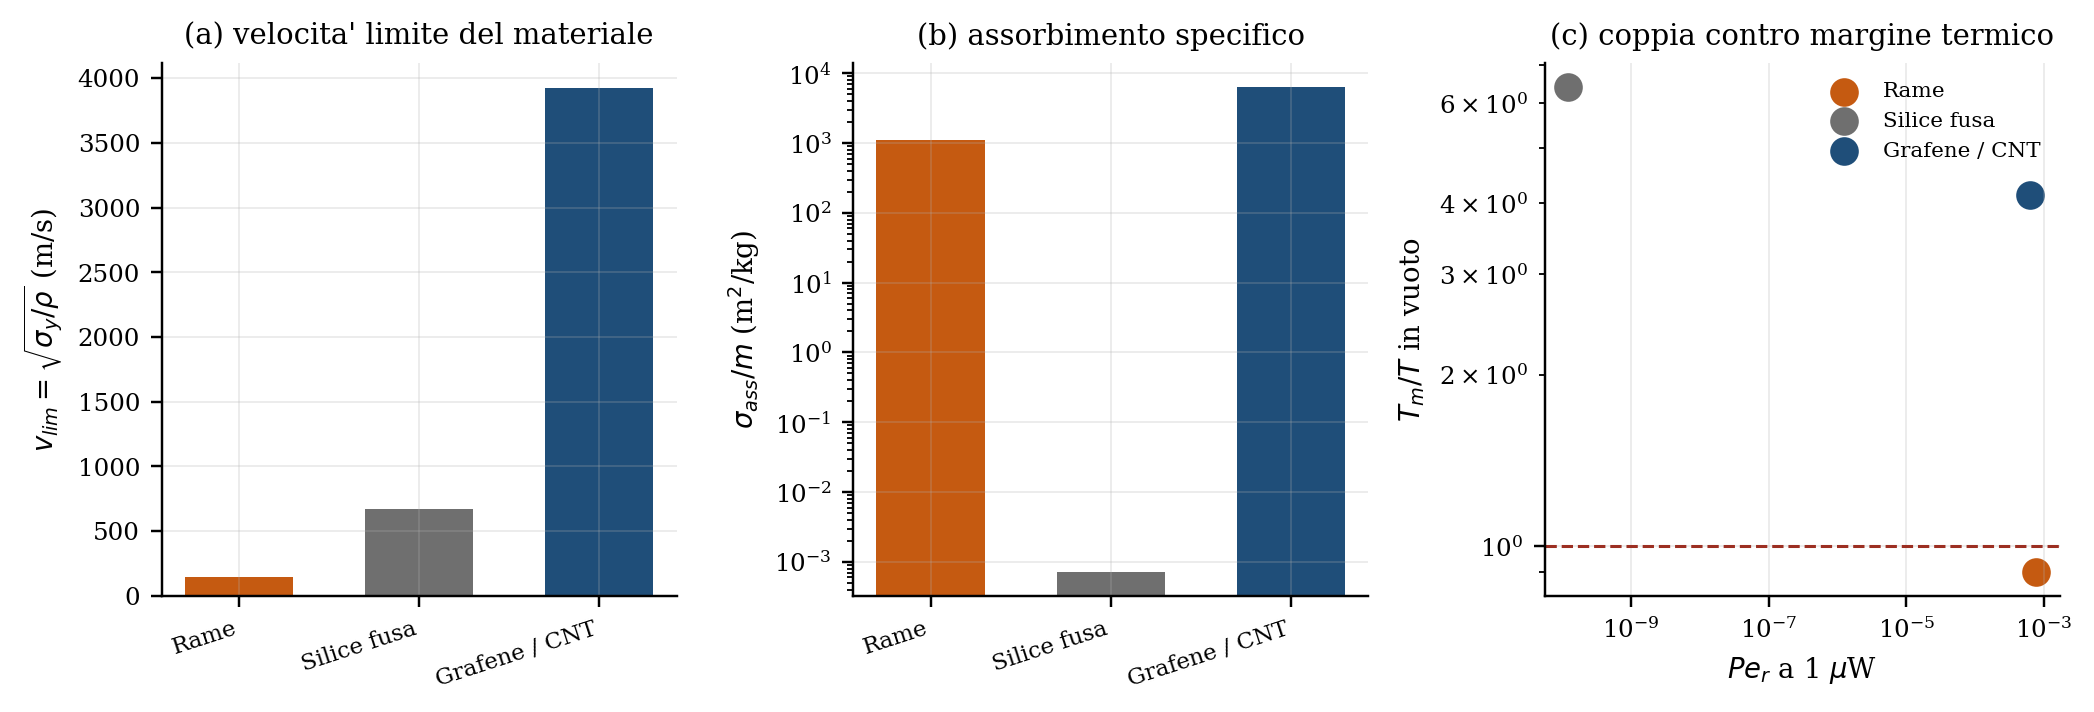
\includegraphics[width=\textwidth]{../figure/fig06_materiali.png}
\caption{\textbf{(a)} Velocit\`a limite $\sqrt{\sigma_y/\rho}$, l'unica grandezza che
governa il tetto di rotazione in vuoto. \textbf{(b)} Assorbimento specifico: il rame
vince. \textbf{(c)} Il compromesso reale: chi ha pi\`u coppia ha meno margine termico.}
\label{fig:materiali}
\end{figure}

Il rame vince sull'assorbimento specifico di un fattore 1{,}2 sul grafene e di
$10^{10}$ sulla silice; il grafene vince sulla velocit\`a limite di un fattore 26 sul
rame; la silice vince sui margini termici e perde su tutto il resto. Non esiste un
materiale migliore: esiste il materiale giusto per il canale scelto.

Per il grafene la voce ``assorbimento'' va maneggiata con cura. Un foglio assorbe il
$2{,}3$\,\% per passaggio ($\pi\alpha$), e una struttura di pochi strati arriva a un
assorbimento confrontabile con il rame; ma la conducibilit\`a termica nel piano \`e
\SI{3000}{W/m/K} contro \SI{401}{W/m/K}, e il gradiente interno, trascurabile per il
rame, qui va calcolato. La V6 usa una densit\`a efficace di
1300\,kg/m\textsuperscript{3} e una tensione efficace di \SI{20}{GPa}: sono valori di
lavoro, non misure, e vanno sostituiti con dati del singolo campione.

%=====================================================================
\section{Leve di progetto}
\label{sec:leve}
%=====================================================================

\begin{tabular}{p{6.2cm}rrp{5.2cm}}
\hline
Leva & su $Pe_r$ & su $\omega_{ss}$ & nota \\
\hline
Potenza x10 (1 $\to$ 10 $\mu$W) & $10$ $\times$ & $10$ $\times$ &  \\
Messa a fuoco NA 0,9 ($w_0$ 500 $\to$ 361 nm) & $1{,}92$ $\times$ & $1{,}92$ $\times$ &  \\
Polarizzazione lineare (s = 0) & $0$ $\times$ & $0$ $\times$ &  \\
OAM $\ell = 5$ con $s = 1$ (con sovrapposizione) & $1{,}05$ $\times$ & $1{,}05$ $\times$ &  \\
Compattazione a pari massa ($R/10$) & $1$ $\times$ & $290$ $\times$ & coppia invariante; omega per il rapporto degli attriti (1e2-1e3) \\
Vuoto spinto ($p = 10^{-6}$ mbar) & $1$ $\times$ & $1{,}33\times10^{10}$ $\times$ & nessuno stato stazionario reale: il limite diventa la rottura \\
Materiale: grafene invece di rame & $0{,}818$ $\times$ & $0{,}818$ $\times$ & cambia l’assorbimento specifico; effetto su $Pe_r$ $= 0.82$ \\
\hline
\end{tabular}


\begin{figure}[H]
\centering
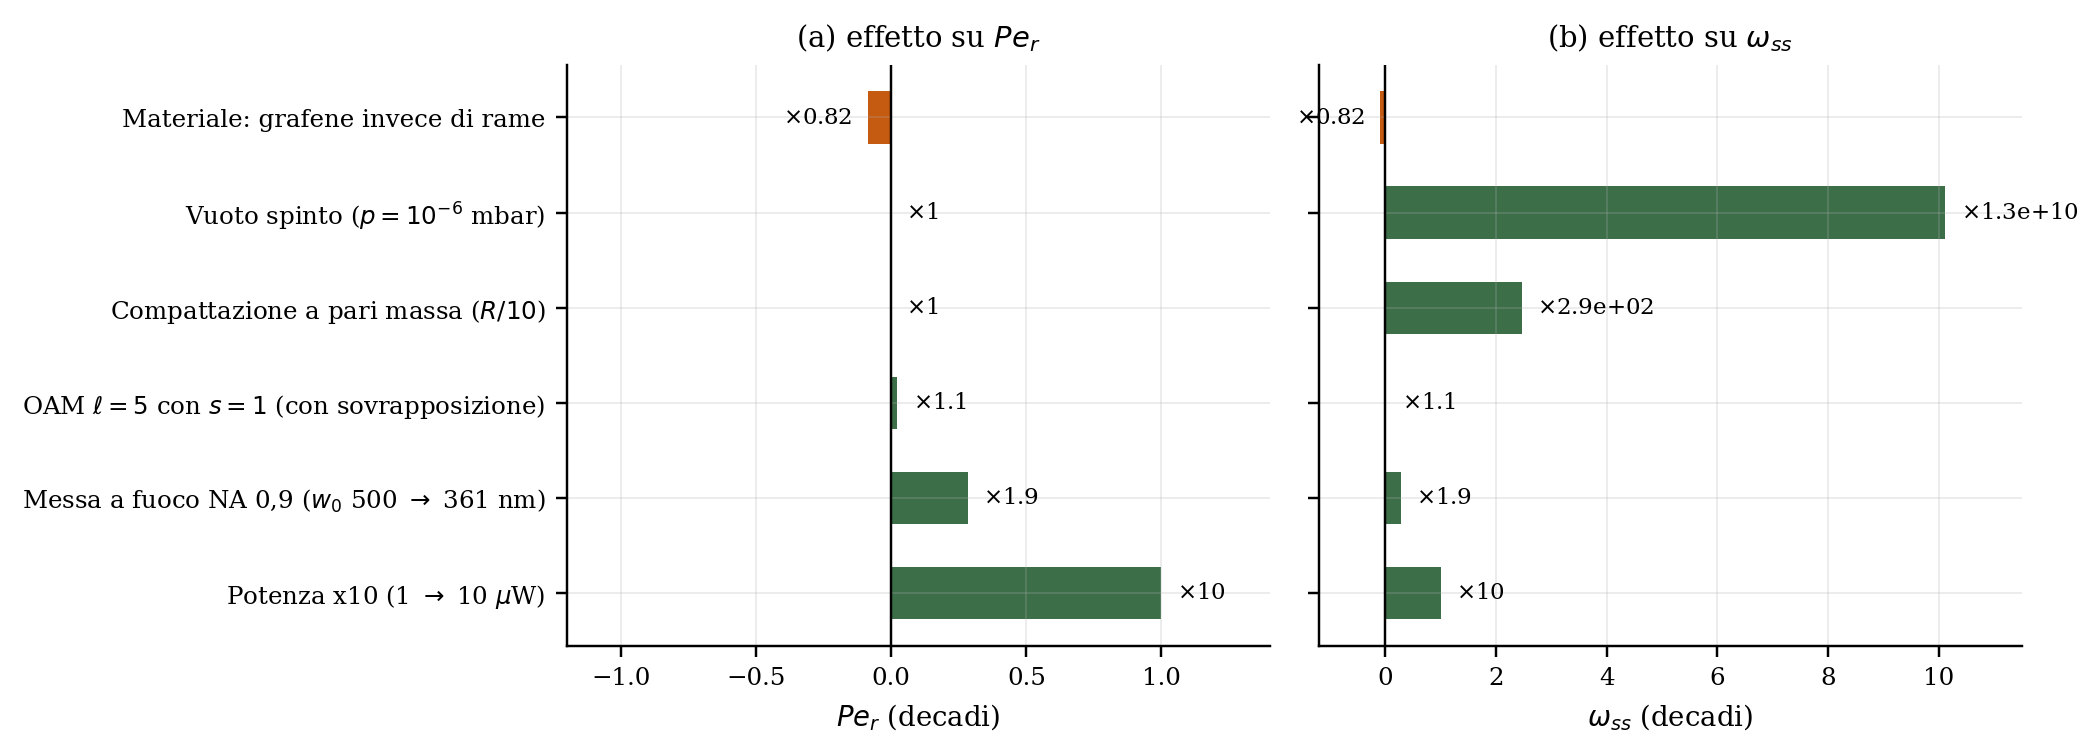
\includegraphics[width=\textwidth]{../figure/fig07_leve.png}
\caption{Effetto di ciascuna leva su $Pe_r$ (a) e su $\omega_{\rm ss}$ (b). Le due
colonne non coincidono, e la differenza \`e il messaggio: compattazione e vuoto
cambiano $\omega$ di dieci decadi e $Pe_r$ di zero.}
\label{fig:leve}
\end{figure}

La leva pi\`u efficace \`e la potenza, e non \`e una sorpresa: $Pe_r\propto P$. La
seconda \`e la messa a fuoco, \SI{1.92}{}; la terza il materiale, che per\`o gioca
contro (il grafene assorbe $0{,}82$ del rame a parit\`a di geometria). L'OAM, come
mostra il \S\ref{sec:oam}, vale $1{,}05$ e non $6$: la tabella lo riporta gi\`a con
la sovrapposizione di modo, ed \`e la correzione pi\`u importante rispetto alla 6.0.

Le due leve ``gratis'' non esistono. La polarizzazione \`e necessaria, non
moltiplicativa: con $s=0$ e $\ell=0$ la coppia \`e zero. La compattazione vale un
fattore 290 su $\omega_{\rm ss}$ e zero su $Pe_r$: migliora la risposta senza
migliorare la forzante, ed \`e esattamente ci\`o che serve a un sensore.

%=====================================================================
\section{Controllo esterno: la silice a 1--6\,GHz}
\label{sec:ghz}
%=====================================================================

Questa sezione non rivendica una validazione. Separa due affermazioni che la 6.0
teneva insieme: la compatibilit\`a di ordine di grandezza sulla \emph{scala
meccanica}, e la validazione del \emph{modello ottico}. La prima \`e verificata, la
seconda no, e nessun dato disponibile la sostiene.

\begin{table}[H]
\centering\small
\caption{Tetto meccanico $f_{\rm lim}=(2\pi r)^{-1}\sqrt{\sigma_y/\rho}$ in GHz, per
quattro raggi e cinque valori della tensione di rottura della silice.}
\label{tab:ghz}
\begin{tabular}{rrrrr}
\hline
$\sigma_y$ (GPa) & $r=25$ nm & $r=50$ nm & $r=75$ nm & $r=100$ nm \\
\hline
0.5 & $3{,}03$ & $1{,}52$ & $1{,}01$ & $0{,}759$ \\
1 & $4{,}29$ & $2{,}15$ & $1{,}43$ & $1{,}07$ \\
3 & $7{,}43$ & $3{,}72$ & $2{,}48$ & $1{,}86$ \\
5 & $9{,}6$ & $4{,}8$ & $3{,}2$ & $2{,}4$ \\
8 & $12{,}1$ & $6{,}07$ & $4{,}05$ & $3{,}03$ \\
\hline
\end{tabular}

\end{table}

\begin{table}[H]
\centering\small
\caption{Le registrazioni sperimentali e la tensione efficace che implicano,
$\sigma_y=\rho(2\pi rf)^2$ con $\rho=2200$\,kg/m$^3$.}
\label{tab:ghz_reg}
\begin{tabular}{rrrr}
\hline
$f$ (GHz) & $r$ (nm) & $v=2\pi r f$ (m/s) & $\rho v^2$ (GPa) \\
\hline
1 & 50 & 314 & 0{,}22 \\
1 & 75 & 471 & 0{,}49 \\
5 & 50 & 1571 & 5{,}43 \\
6 & 50 & 1885 & 7{,}82 \\
\hline
\end{tabular}

\end{table}

\begin{figure}[H]
\centering
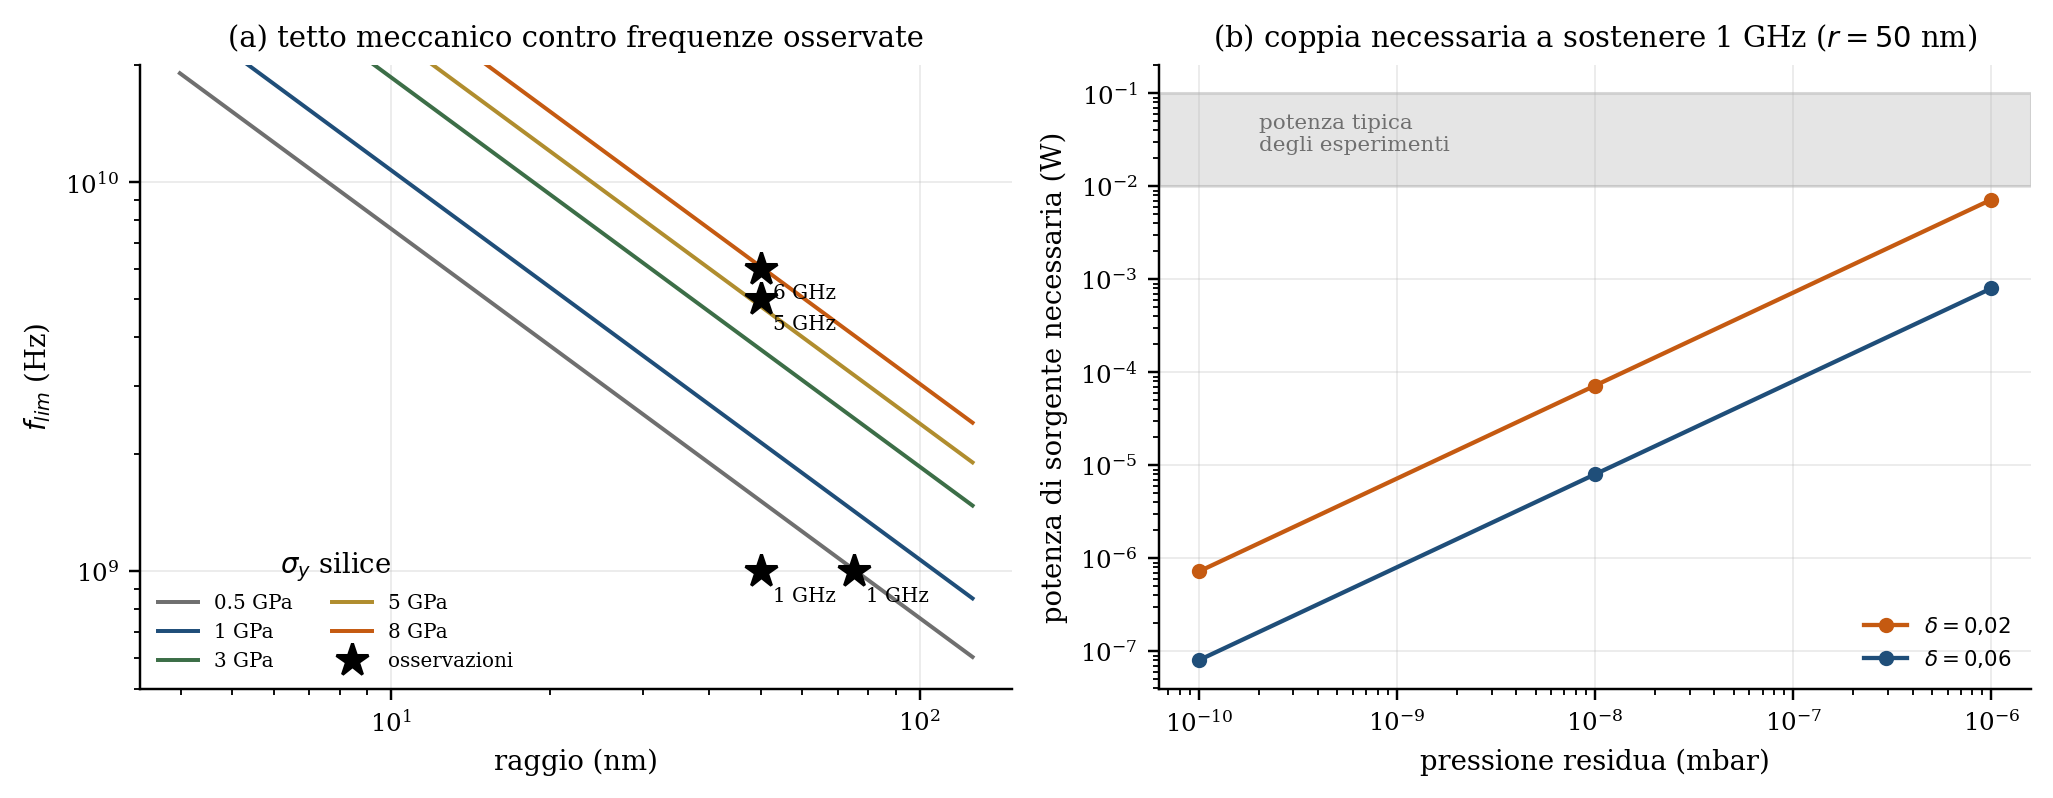
\includegraphics[width=\textwidth]{../figure/fig08_ghz.png}
\caption{\textbf{(a)} Tetto meccanico $f_{\rm lim}=(2\pi r)^{-1}\sqrt{\sigma_y/\rho}$
per cinque valori di $\sigma_y$; le stelle sono le frequenze osservate. Le
osservazioni cadono fra 0,2 e 8\,GPa, cio\`e nell'intervallo della silice su
nanoscala. \textbf{(b)} Potenza di sorgente necessaria a sostenere \SI{1}{GHz} contro
l'attrito molecolare: molto sotto la potenza impiegata negli esperimenti, che serve
alla trappola, non alla coppia.}
\label{fig:ghz}
\end{figure}

\textbf{(1) Compatibilit\`a meccanica.} Le coppie $(f,r)$ riportate implicano
$\sigma_y$ fra $0{,}22$\,GPa (\SI{1}{GHz} a \SI{50}{nm}) e $7{,}8$\,GPa
(\SI{6}{GHz} a \SI{50}{nm}). La formula riproduce le frequenze osservate per valori
di $\sigma_y$ che sono quelli attesi per la silice su nanoscala, e questo \`e un
controllo di coerenza, non una previsione: $\sigma_y$ \`e stato ricavato dalle
osservazioni, non misurato indipendentemente. Un solo punto, con $\sigma_y$ scelto,
non \`e una validazione; quattro punti con $\sigma_y$ libero sono un vincolo.

\textbf{(2) La coppia \`e sovrabbondante.} A \SI{1}{GHz} in vuoto a
\SI{1e-6}{mbar} l'attrito molecolare su una sfera di \SI{50}{nm} vale
$1{,}0\times10^{-27}$\,N\,m; servono \SI{0.8}{mW} di sorgente con $\delta=0{,}06$ e
\SI{8}{\micro W} a \SI{1e-8}{mbar}, contro i \SI{10}{}--\SI{100}{mW} tipici. La
differenza \`e la trappola ottica. Il modello prevede coppia in eccesso, e questo \`e
coerente con l'esperimento, ma non lo dimostra.

\textbf{(3) Ci\`o che manca per parlare di validazione.} Servirebbe il confronto di
$\tau$ misurata contro $P_{\rm ass}$ a geometria nota, e la dipendenza di
$\omega_{\rm ss}$ da $\beta$ a mezzo variabile. Nessuno dei due \`e disponibile per
questo dispositivo. La frase corretta \`e quindi: il confronto offre un controllo
esterno preliminare sulla scala meccanica, non una validazione sperimentale del
Motore Fotonico.

%=====================================================================
\section{OAM come analisi di sensibilit\`a}
\label{sec:oam}
%=====================================================================

La 6.0 trattava $\ell$ come un moltiplicatore: $\tau=(\ell+s)P_{\rm ass}/\omega_{\rm
ott}$, quindi $\ell=5$ vale sei volte. \`E sbagliato a potenza \emph{incidente}
fissata, perch\'e $\eta_{\rm int}$ non resta costante.

Per un fascio $LG_{0\ell}$ di potenza $P$ e waist $w_0$ l'intensit\`a di picco,
normalizzata a quella gaussiana, vale
\begin{equation}
g(\ell)=\frac{\ell^{\ell}e^{-\ell}}{\ell!},
\qquad g(1)=0{,}368,\; g(5)=0{,}176,\; g(10)=0{,}125,
\end{equation}
e sull'asse \`e nulla per $\ell\ge1$. Una particella posta sul massimo intercetta
$\sigma I_{\rm picco}$, quindi la coppia netta scala come $(\ell+s)\,g(\ell)$:
\begin{center}\small
\begin{tabular}{lrrrrr}
\toprule
$\ell$ & 0 & 1 & 5 & 10 & 20 \\
\midrule
$g(\ell)$ & 1 & 0,368 & 0,176 & 0,125 & 0,089 \\
$\tau(\ell)/\tau(0)$ & 1 & 0,74 & 1,05 & 1,38 & 1,87 \\
\bottomrule
\end{tabular}
\end{center}
Il guadagno \`e dell'ordine di $\sqrt{\ell}$, non di $\ell$, e per $\ell=1$ \`e
addirittura una perdita. C'\`e per\`o un vantaggio pratico che la V6 registra e non
quantifica: un fascio con $\ell\neq0$ porta il momento angolare in una regione
anulare, e questo permette di far passare la luce di trappola al centro e quella di
coppia sull'anello. \`E una ragione di progetto, non una ragione fisica, e va
verificata misurando $\eta_{\rm int}(\ell)$.

\begin{figure}[H]
\centering
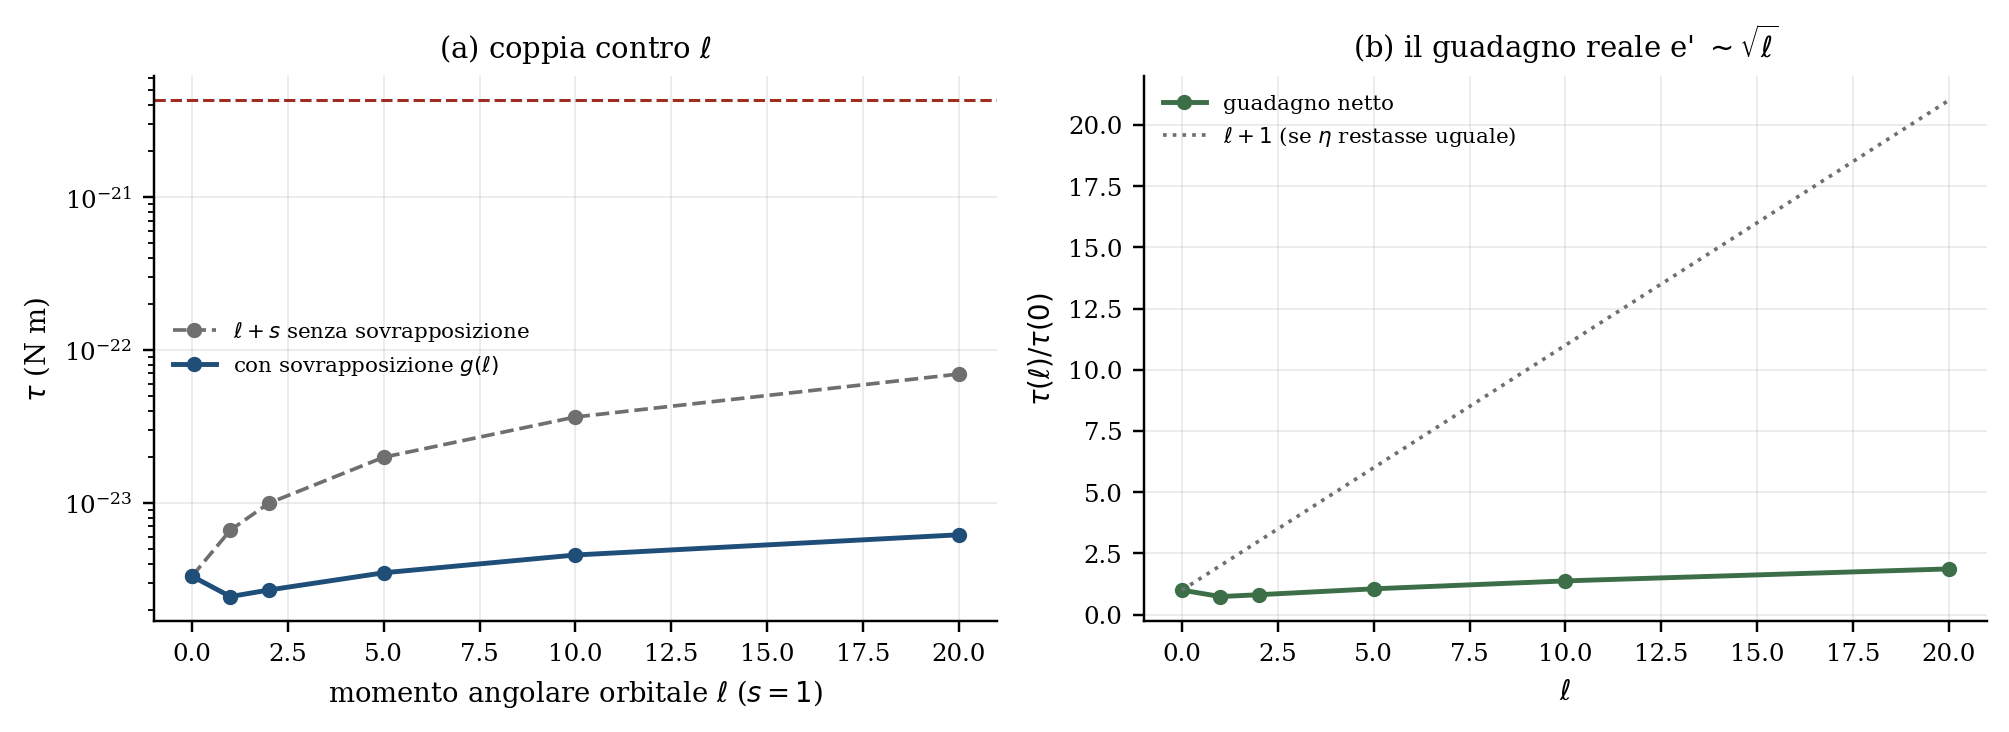
\includegraphics[width=\textwidth]{../figure/fig09_oam.png}
\caption{\textbf{(a)} Coppia contro $\ell$ con e senza la sovrapposizione di modo.
\textbf{(b)} Guadagno netto: la curva grigia \`e ci\`o che si otterrebbe se $\eta$
restasse costante, quella verde \`e ci\`o che si ottiene.}
\label{fig:oam}
\end{figure}

%=====================================================================
\section{Limiti, falsificabilit\`a, protocollo}
\label{sec:limiti}
%=====================================================================

\subsection{Cosa la V6 non ha fatto}
\begin{enumerate}\itemsep2pt
\item \textbf{Calcolo full-wave dell'intero telaio.} La sovrapposizione \`e
incoerente e dichiarata; un DDA/FDTD pu\`o cambiare $\sigma_{\rm pr}$ di un fattore 4.
\`E il primo lavoro da fare, e condiziona l'intera sezione sulla coppia.
\item \textbf{Ottica per forma.} Disco, anello e manubrio hanno una banda, non un
valore. Senza DDA la loro $Pe_r$ resta condizionale.
\item \textbf{Accoppiamento termo-meccanico.} La temperatura \`e calcolata in regime
stazionario su un corpo rigido; la dilatazione differenziale fra nucleo e telaio e la
perdita di planarit\`a non sono trattate.
\item \textbf{Contro-spin dinamico.} Il rapporto 45/376 \`e trattato come vincolo
cinematico; la dinamica del vincolo non \`e calcolata.
\item \textbf{Fluido reale.} Acqua newtoniana a \SI{20}{\degreeCelsius}; un mezzo
biologico \`e viscoelastico.
\end{enumerate}

\subsection{Come smentire la V6}
\begin{enumerate}\itemsep2pt
\item \textbf{Coppia contro potenza assorbita.} La \eqref{eq:modello} prevede
$\tau/P_{\rm ass}=1/\omega_{\rm ott}=2{,}82\times10^{-16}$\,s. Se una misura su una
particella di rame di \SI{40}{nm} la supera, il modello \`e incompleto e il canale di
scattering trasferisce momento angolare in modo coerente.
\item \textbf{Dipendenza da $\beta$.} La \eqref{eq:identita} prevede che $Pe_r$ non
cambi passando da acqua ad acqua-glicole mentre $\omega_{\rm ss}$ scala come
$1/\beta$. Se $Pe_r$ cambia, il modello di attrito \`e sbagliato.
\item \textbf{Soglia termica in vuoto.} La V6 prevede fusione a
\SI{0.13}{}--\SI{0.66}{\micro W}. Se la fusione avviene a potenza molto pi\`u alta, il
bilancio radiativo \`e incompleto (conduzione attraverso il mezzo di levitazione) o
l'area \`e molto maggiore di quella geometrica.
\end{enumerate}

\subsection{Protocollo per l'audit full-wave}
\begin{itemize}\itemsep1pt
\item Geometria: telaio V5 esatto, fili 6,4 / 15 / 9 nm, nucleo \SI{40}{nm}.
\item Materiale: rame con $\varepsilon(a)$ di Drude, pi\`u guscio di Cu$_2$O di
0, 1, 2 nm.
\item Discretizzazione: passo $\le\lambda/20$ nel metallo ($\le\SI{13}{nm}$), con
verifica di convergenza a due passi.
\item Incidenza: quattro orientazioni, polarizzazione circolare.
\item Uscita: $\sigma_{\rm ext}$, $\sigma_{\rm abs}$, $g$, $\sigma_{\rm pr}$, e il
confronto con la somma incoerente usata qui.
\end{itemize}

%=====================================================================
\appendix
\section{Il ciclo a 720$^\circ$ e il rapporto 45/376}
\label{app:su2}
%=====================================================================

Questo materiale va conservato, non promosso. Tre affermazioni, in ordine di
solidit\`a decrescente.

\textbf{Prima, solida.} La scena della V5 compie 720$^\circ$ sullo Spin e
86{,}1702$^\circ$ sul Contro-spin in 240 fotogrammi, con chiavi assolute e nessuna
riduzione modulo 360. \`E un fatto verificabile nel file \texttt{.blend} e nel codice.

\textbf{Seconda, convenzionale.} La copertura doppia di $SO(3)$ \`e una propriet\`a di
$SU(2)$: $U(\theta)=\exp(-i\theta\sigma_z/2)$ cambia segno a $2\pi$ e torna a $+1$ a
$4\pi$. Un rotore \`e un corpo macroscopico e la sua periodicit\`a geometrica \`e
$2\pi$; la periodicit\`a a $4\pi$ \`e una scelta di costruzione dell'animazione, non
una firma misurabile.

\textbf{Terza, da non usare.} Il rapporto $I_2/I_1=45/376$ chiude la cinematica, non
la dinamica. La V5 otteneva la chiusura aggiungendo $3{,}06\times10^{-20}$\,kg a
\SI{42}{nm} dal centro ($2{,}9\times10^5$ atomi di rame, l'$1{,}1$\,\% della massa del
telaio). La V6 non usa quella massa: il punto di applicazione cade dentro il nucleo e
non corrisponde a nessun elemento della scena. E soprattutto nulla garantisce che le
coppie ottiche e dissipative producano spontaneamente quel rapporto. Un rapporto
razionale fra due velocit\`a angolari garantisce la ripetizione geometrica \emph{se}
il rapporto viene mantenuto; il mantenimento richiede un vincolo meccanico, e un
vincolo meccanico fra i due rotori li rende un unico corpo rigido, con un solo momento
d'inerzia. Il Contro-spin non pu\`o essere contemporaneamente indipendente (per avere
un rapporto proprio) e vincolato (per mantenerlo).

Il rapporto 45/376 resta una propriet\`a della forma, invariante su nove ordini di
grandezza di scala e sui tre materiali. Come tale va citato, senza la massa di
bilanciamento e senza l'aura quantistica che la V4 gli attribuiva.

\begin{figure}[H]
\centering
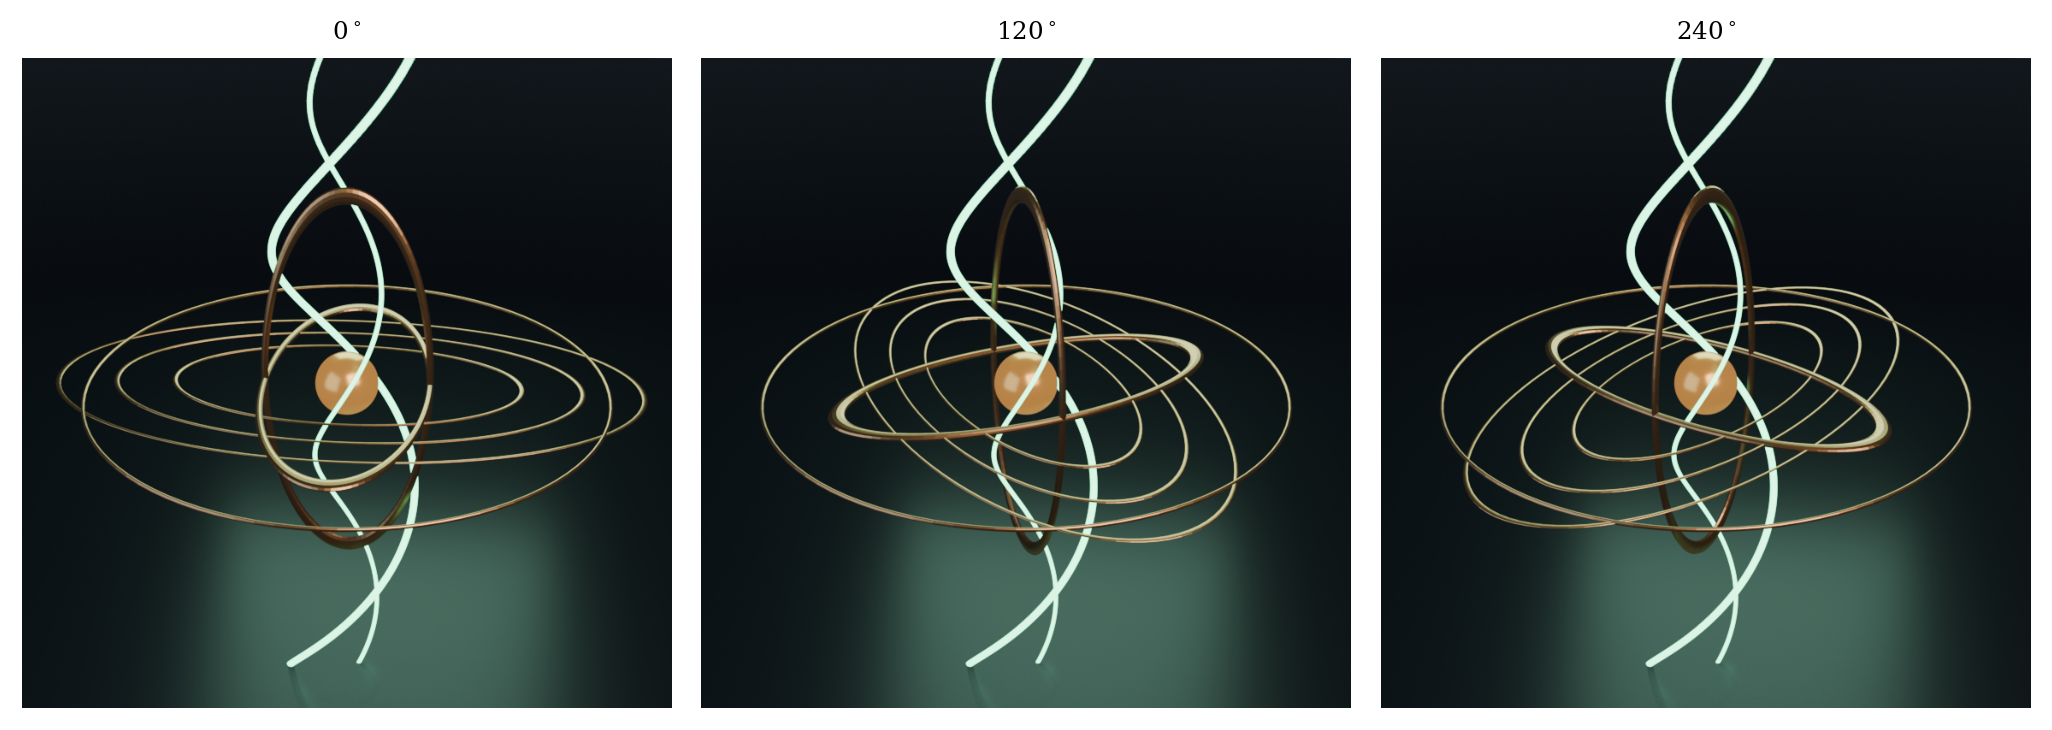
\includegraphics[width=\textwidth]{../figure/fig12_sequenza.png}
\caption{Tre orientazioni della scena a 0, 120 e 240$^\circ$. L'animazione \`e una
verifica di coerenza geometrica del ciclo, non una simulazione fisica.}
\label{fig:sequenza}
\end{figure}

\section{Materiale escluso e suo destino}

Due temi della V5 non entrano nella V6, e non \`e una dimenticanza. L'\emph{arca} e il
\emph{sangue} --- le metafore cosmologiche e il riferimento al mezzo biologico come
giustificazione del progetto --- appartengono a un altro discorso, e mescolarli a
un'analisi dimensionale indebolisce entrambi: vanno in un testo separato. La
\emph{modalit\`a pulsata} resta, ma declassata a leva termica
(\S\ref{sec:termica}): la costante di tempo meccanica di \SI{1.1}{ns} rende impossibile
che la pulsazione cambi la dinamica.

\section{Codice, dati e riproducibilit\`a}

Ogni numero del testo viene da uno di quattro script, che non contengono dati scritti
a mano.

\begin{center}\small
\begin{tabular}{p{3.4cm}p{9.4cm}}
\toprule
file & funzione \\
\midrule
\texttt{v6\_nucleo.py} & ottica (Mie, cilindro, core-shell), attrito, termica,
dinamica; self-test \\
\texttt{v6\_studi.py} & i nove studi, i JSON in \texttt{dati/}, le tabelle in
\texttt{tabelle/} \\
\texttt{v6\_figure.py} & le dodici figure dai record di calcolo \\
\texttt{v6\_blender.py} & la scena e i render in \texttt{blender/} \\
\bottomrule
\end{tabular}
\end{center}

Il self-test verifica la convergenza della serie cilindrica contro Rayleigh, la
conservazione $Q_{\rm ext}\ge Q_{\rm sca}$, l'identit\`a \eqref{eq:identita} e i
limiti della sfera rivestita. Chi vuole contestare un numero deve contestare una di
queste verifiche: \`e il senso della revisione.

\section*{Ringraziamenti}
\addcontentsline{toc}{section}{Ringraziamenti}
La revisione nasce da una critica esterna che ha indicato i residui, la struttura in
cinque fasi, il criterio in quattro domande e, nella 6.1, i cinque errori materiali
corretti qui: raggi dei fili, numero $0{,}119667646$, area radiante, circolarit\`a
della baseline e punto singolo nel confronto a GHz. La V6 \`e un'esecuzione di quel
programma.

\begin{thebibliography}{9}\small
\bibitem{bh} C.~F. Bohren, D.~R. Huffman, \emph{Absorption and Scattering of Light
by Small Particles}, Wiley, New York, 1983, cap.~4 (sfera), cap.~5 (sfera
rivestita), cap.~8 (cilindri).
\bibitem{jc} P.~B. Johnson, R.~W. Christy, Optical constants of the noble metals,
\emph{Phys. Rev. B} \textbf{6}, 4370--4379 (1972).
\bibitem{kerker} M.~Kerker, \emph{The Scattering of Light and Other Electromagnetic
Radiation}, Academic Press, New York, 1969, cap.~5 (Maxwell-Garnett).
\bibitem{ll} L.~D. Landau, E.~M. Lifshitz, \emph{Fluid Mechanics}, 2nd ed.,
Pergamon, 1987, \S\,20: disco che ruota attorno al proprio asse,
$M=(32/3)\mu R^3\Omega$.
\bibitem{cox} R.~G. Cox, The motion of long slender bodies in a viscous fluid,
\emph{J. Fluid Mech.} \textbf{44}, 791--810 (1970).
\bibitem{bat} G.~K. Batchelor, Slender-body theory for particles of arbitrary
cross-section in Stokes flow, \emph{J. Fluid Mech.} \textbf{44}, 419--440 (1970).
\bibitem{nair} R.~R. Nair et al., Fine structure constant defines visual
transparency of graphene, \emph{Science} \textbf{320}, 1308--1310 (2008).
\bibitem{marston} P.~L. Marston, J.~H. Crichton, Radiation torque on a sphere caused
by a circularly-polarized electromagnetic wave, \emph{Phys. Rev. A} \textbf{30},
2508--2516 (1984).
\bibitem{reimann} R.~Reimann et al., GHz rotation of an optically trapped nanoparticle
in vacuum, \emph{Phys. Rev. Lett.} \textbf{121}, 033602 (2018).
\bibitem{ahn} J.~Ahn et al., Ultrasensitive torque detection with an optically
levitated nanorotor, \emph{Nat. Nanotechnol.} \textbf{15}, 89--93 (2020).
\bibitem{v5} F.~Bulla, \emph{Motore Fotonico del Vuoto V5}, preprint, 2026
(documento di provenienza di tutti i valori citati come ``V5'').
\end{thebibliography}

\end{document}
